\pdfobjcompresslevel=0
\documentclass[11pt]{saim}
% Common math shortcuts for the template.
\usepackage{amsmath,amssymb,amsfonts,amsthm,mathtools,bm}

\newcommand{\R}{\mathbb{R}}
\newcommand{\E}{\mathbb{E}}
\newcommand{\Var}{\mathrm{Var}}
\newcommand{\Cov}{\mathrm{Cov}}
\newcommand{\KL}{\mathrm{KL}}
\newcommand{\norm}[1]{\left\lVert #1 \right\rVert}
\newcommand{\abs}[1]{\left\lvert #1 \right\rvert}
\newcommand{\set}[1]{\left\{ #1 \right\}}
\newcommand{\paren}[1]{\left( #1 \right)}
\newcommand{\bracket}[1]{\left[ #1 \right]}
\newcommand{\ip}[2]{\left\langle #1, #2 \right\rangle}
\newcommand{\myeq}{\stackrel{\mathclap{\small\mbox{def}}}{=}}

\newtheorem{theorem}{Theorem}[section]
\newtheorem{lemma}[theorem]{Lemma}
\newtheorem{proposition}[theorem]{Proposition}
\newtheorem{corollary}[theorem]{Corollary}
\newtheorem{assumption}[theorem]{Assumption}
\theoremstyle{definition}
\newtheorem{definition}[theorem]{Definition}
\newtheorem{remark}[theorem]{Remark}

% ----- HAVI-Methyl extensions -----
\providecommand{\LN}{\mathrm{LogitNormal}}
\providecommand{\Bet}{\mathrm{Beta}}
\providecommand{\BB}{\mathrm{BetaBin}}
\providecommand{\NB}{\mathrm{NegBin}}
\providecommand{\Cat}{\mathrm{Cat}}
\providecommand{\Dir}{\mathrm{Dir}}
\providecommand{\sigm}{\sigma}
\providecommand{\logit}{\mathrm{logit}}
\providecommand{\bbeta}{\boldsymbol{\beta}}
\providecommand{\bdelta}{\boldsymbol{\delta}}
\providecommand{\btheta}{\boldsymbol{\theta}}
\providecommand{\bphi}{\boldsymbol{\phi}}
\providecommand{\bpi}{\boldsymbol{\pi}}
\providecommand{\bz}{\mathbf{z}}
\providecommand{\elbo}{\mathcal{L}}
\providecommand{\N}{\mathcal{N}}


% ----- Additional packages required by the manuscript -----
\usepackage{url}
\usepackage{enumitem}
\usepackage{graphicx}
\usepackage{float}
\usepackage[ruled,vlined,linesnumbered]{algorithm2e}
\usepackage{longtable,tabularx}
\usepackage{listings}
\usepackage{tikz}
\usetikzlibrary{bayesnet,positioning,fit,arrows.meta}

% ----- Listings style for code blocks -----
\definecolor{codegray}{RGB}{120,120,120}
\definecolor{codeaccent}{RGB}{50,18,122}
\lstdefinestyle{py}{
  basicstyle=\ttfamily\footnotesize,
  keywordstyle=\color{codeaccent},
  commentstyle=\color{codegray}\itshape,
  stringstyle=\color{black},
  language=Python,
  showstringspaces=false,
  breaklines=true,
  frame=single,
  rulecolor=\color{codegray!50},
  numbers=left,
  numberstyle=\tiny\color{codegray}
}

% ----- Takeaway-box environment for highlighted callouts -----
\newtcolorbox{takeawaybox}{
  enhanced,
  colback=saimbg!40,
  colframe=saimindigo!70,
  boxrule=0.5pt,
  arc=2pt,
  left=8pt,
  right=8pt,
  top=6pt,
  bottom=6pt,
  before skip=6pt,
  after skip=6pt
}

% ----- Title block metadata -----
\title{HAVI-Methyl: Hierarchical Amortized Variational Inference\\for Methylation Prediction from Cell-Free DNA Fragmentomics}
\author[1]{Omid Shams Solari}
\affiliation[1]{sAIm Labs}
\correspondence{\email{omid.solari@saimai.com}}

\abstract{%
\textbf{Problem.} Cell-free DNA (cfDNA) whole-genome sequencing has become the dominant non-invasive substrate for non-invasive prenatal testing, minimal residual disease monitoring, and early cancer detection, but methylation information remains expensive to access because bisulfite conversion is destructive and biased. \citet{liu2024finaleme} closed part of this gap with FinaleMe, a per-sample two-state hidden Markov model that recovers methylation from fragmentomic features alone. Its binary latent state, point-estimate Baum-Welch fit, per-sample training, susceptibility to prior leakage, lower-information CpG regimes, and binarized downstream tissue deconvolution leave room for a fully probabilistic successor.

\smallskip\textbf{Method.} We present \textbf{HAVI-Methyl} (Hierarchical Amortized Variational Inference for Methylation), a hierarchical Bayesian framework for methylation prediction from cfDNA fragmentomics. The full proposed model uses a population locus prior $\beta^{\mathrm{pop}}_\ell$, a per-sample shift $\delta_s$, and a per-(sample, locus) latent $\beta_{s,\ell}$ on the logit scale, with direct-count, pseudo-count, end-motif, and coverage likelihoods chosen according to the observation regime. Inference is designed as stochastic variational inference with approximate moment-matched natural-gradient updates on the population layer and an amortized normalizing-flow variational posterior $q_\phi(\eta_{s,\ell}\mid F_{s,\ell})$ over per-locus fragment bags, encoded by a permutation-invariant Set Transformer and optional frozen long-range DNA embeddings. Prior-leakage control is handled by a variational information-bottleneck penalty, mQTL anchor losses, and counterfactual augmentation. Calibrated prediction sets come from posterior-predictive checks plus a split-conformal wrapper, and the proposed tissue-of-origin module uses posterior methylation uncertainty rather than binarized point estimates.

\smallskip\textbf{Results.} The completed experiments in this manuscript are synthetic experiments from the released simplified harness, not a completed full real-data benchmark. On 12 simulated samples and 300 loci across coverages $\{0.1\times,1\times,5\times,30\times\}$, the simplified HAVI-Methyl variant achieves Pearson $r$ of $0.333$ / $0.782$ / $0.868$ / $0.964$ versus a FinaleMe-style HMM baseline at $0.162$ / $0.524$ / $0.768$ / $0.961$, with consistent RMSE reductions and stronger recovery on a synthetic low-information locus proxy. In a synthetic prior-leakage stress test, VIB reduces prior attribution from $5.9\%$ to $0.6\%$ of the predicted DMR signal, and adding mQTL anchors reduces it to $0.04\%$. A simplified continuous deconvolution proxy reduces synthetic tissue-fraction RMSE from $0.129$ to $0.007$; full joint Dirichlet-head evaluation remains part of the planned benchmark.

\smallskip\textbf{Contributions.} We provide ELBO, reparameterization-gradient, and approximate natural-gradient derivations; give formal propositions or proof sketches for lower-bound validity, conditional instrumental-anchor identifiability, VIB-bounded prior leakage, conformal marginal coverage, surrogate SVI convergence, hierarchical-pooling variance reduction, and information-theoretic recoverability limits; and introduce a chromatin-aware cfDNA fragmentation-simulator specification. We preserve the planned real-data benchmarking program against the paired WGS/WGBS data of \citet{liu2024finaleme} and public tissue atlases, with ablations, calibration diagnostics, and compute-planning estimates clearly marked as planned work.
}


\begin{document}
\maketitle

\tableofcontents

\section{Introduction}
\label{sec:intro}

Cell-free DNA (cfDNA) whole-genome sequencing has become the dominant non-invasive substrate for non-invasive prenatal testing (NIPT), minimal residual disease (MRD) monitoring, and early cancer detection \citep{snyder2016,sun2015,moss2018,loyfer2023}. The clinical pipeline produces enormous quantities of low-pass WGS data, but the vast majority of methylation information remains inaccessible because bisulfite conversion is destructive, expensive, and biased toward fragment ends. \citet{liu2024finaleme} closed part of this gap with FinaleMe by showing that fragmentomic features---fragment length, end motifs, GC content, and orientation---are sufficient to recover per-CpG methylation status through a per-sample hidden Markov model. FinaleMe demonstrates genome-wide Pearson correlations that vary by region between roughly $0.5$ in CpG-sparse regions and approximately $0.7$ in CpG-rich regions on $20\times$ low-pass WGS, with substantial degradation at lower coverage and outside CpG islands; we refer the reader to \citet[Fig.~3]{liu2024finaleme} for the full empirical breakdown.

Despite its impact, FinaleMe has well-defined limitations that motivate this work. We list them as seven distinct items, each tied to the corresponding HAVI-Methyl design choice that addresses it.

\paragraph{(L1) Binary latent state.} FinaleMe's hidden state is binary $\{m,u\}$, discarding the continuous $\beta\in[0,1]$ structure that drives all downstream tissue-of-origin and biological-age inference. \emph{HAVI-Methyl response:} a continuous logit-$\beta$ latent with a Beta-Binomial likelihood (Section~\ref{sec:model}).

\paragraph{(L2) No uncertainty quantification.} FinaleMe returns Viterbi point estimates, which is a serious obstacle for clinical deployment where calibrated risk is required. \emph{Response:} a normalizing-flow variational posterior with conformal coverage guarantees (Sections~\ref{sec:varfamily} and~\ref{sec:calibration}).

\paragraph{(L3) Per-sample fitting.} FinaleMe re-runs Baum-Welch from scratch on every sample, ignoring statistical strength shared across thousands of samples in modern biobanks. \emph{Response:} a hierarchical Bayesian model with a population locus prior, fitted by stochastic variational inference (Sections~\ref{sec:model} and~\ref{sec:elbo}).

\paragraph{(L4) Buffy-coat prior leakage.} The prior is seeded from the same individual's leukocyte methylome, so any disease signal that also alters leukocytes (inflammation, treatment effects) is absorbed into the prior and erased from the prediction. \emph{Response:} a variational information-bottleneck penalty, an mQTL-anchor instrumental-variable loss, and counterfactual augmentation (Section~\ref{sec:identify}).

\paragraph{(L5) Poor performance in CpG-poor regions.} The Markov chain along loci forces information to propagate through chromosomal neighbors that themselves lack signal. \emph{Response:} amortized inference over the fragment bag at each locus through a permutation-invariant Set Transformer encoder and a long-range DNA sequence context (Section~\ref{sec:varfamily}).

\paragraph{(L6) Tissue deconvolution on binarized predictions.} FinaleMe's downstream tissue-of-origin pipeline binarizes the per-CpG predictions before solving a quadratic program for tissue fractions, discarding posterior mass and breaking calibration. \emph{Response:} a Dirichlet head on continuous posterior means with optional hierarchical Dirichlet process extension, trained jointly with the methylation ELBO (Section~\ref{sec:too}).

\paragraph{(L7) No inter-fragment pooling.} Beyond the per-fragment HMM emissions, no mechanism aggregates information across fragments at a single locus. \emph{Response:} the Set Transformer pooling step that produces a permutation-invariant locus embedding from the entire fragment bag at once (Section~\ref{sec:varfamily}).

\paragraph{Contributions.} The paper makes the following contributions.

\noindent (i) A complete generative model for cfDNA fragmentomics with a hierarchical logit-Normal prior and Beta-Binomial / Categorical / Negative-Binomial likelihoods (Section~\ref{sec:model}).

\noindent (ii) A full ELBO derivation with approximate natural-gradient updates on the population latents and an amortized neural-spline-flow posterior on the per-(sample, locus) latents, with explicit handling of the non-conjugate natural-gradient correction (Sections~\ref{sec:elbo} and~\ref{sec:algo}).

\noindent (iii) Five formal propositions and two new theoretical contributions, including hierarchical identifiability under instrumental anchors with explicit nonparametric IV completeness, an asymptotic variational-information-bottleneck prior-leakage bound with a finite-$\beta_{\mathrm{VIB}}$ corollary, conformal marginal coverage, convergence of non-conjugate natural-gradient SVI, a hierarchical-pooling variance-reduction inequality, and a Fano-style information-theoretic recoverability lower bound (Section~\ref{sec:theory}).

\noindent (iv) A chromatin-aware cfDNA fragmentation simulator that generates paired ground-truth methylation and WGS reads (Section~\ref{sec:simulator} and Appendix~\ref{app:sim}).

\noindent (v) Synthetic recovery experiments with reproducible code (Section~\ref{sec:synth}).

\noindent (vi) A benchmarking plan against FinaleMe on the 80 paired WGS/WGBS samples and the Sun, Moss, and Loyfer reference atlases, with full ablations (Section~\ref{sec:benchmark}).

\noindent (vii) A wafer-scale accelerator training recipe with parameter-count and FLOP estimates exploiting wafer-scale weight streaming for genome-wide locus mini-batching (Section~\ref{sec:benchmark}).

\paragraph{Relationship to methylation foundation models.} HAVI-Methyl complements rather than competes with the recent foundation-model line of work on methylation, of which CpGPT \citep{cpgpt2024} and MethylGPT \citep{methylgpt2024} are the leading examples. Foundation models consume per-CpG $\beta$-values from methylation arrays as input and produce embeddings or downstream predictions; HAVI-Methyl consumes raw cfDNA WGS fragments and produces $\beta$-values as output. The two pipelines compose: HAVI-Methyl provides the input to a foundation model, and the foundation model provides downstream embeddings, biological-age clocks (PhenoAge, GrimAge, DunedinPACE, PC-clocks; \citealp{horvath2013,levine2018phenoage,lu2019grimage,belsky2022dunedinpace,higginschen2022pcclocks}), or imputation of missing CpGs. Section~\ref{sec:related} expands on this relationship.

\paragraph{Roadmap.} Section~\ref{sec:background} reviews cfDNA fragmentomics, variational Bayesian inference, and the methylation-clock and foundation-model literature. Section~\ref{sec:model} specifies the generative model. Section~\ref{sec:varfamily} defines the structured variational family. Section~\ref{sec:elbo} derives the ELBO with all reparameterization, IWAE, mini-batch rescaling, and natural-gradient details. Section~\ref{sec:algo} states the SVI training algorithm. Section~\ref{sec:identify} establishes identifiability through the VIB penalty, mQTL anchors, counterfactual augmentation, and domain-adversarial training. Section~\ref{sec:calibration} derives the conformal calibration wrapper. Section~\ref{sec:too} attaches the joint tissue-of-origin head. Section~\ref{sec:simulator} introduces the cfDNA simulator. Section~\ref{sec:synth} reports synthetic recovery results. Section~\ref{sec:benchmark} lays out the benchmarking plan on real data. Section~\ref{sec:theory} collects the seven formal propositions. Section~\ref{sec:discussion} discusses limitations and extensions. Section~\ref{sec:related} treats related work in detail. Section~\ref{sec:conc} concludes. Appendices~\ref{app:elbo}--\ref{app:extres} contain full derivations, the VB-HMM baseline updates, simulator validation, hyperparameter tables, the notation glossary, and extended results.

\section{Background and Preliminaries}
\label{sec:background}

\subsection{cfDNA fragmentomics}
cfDNA fragments are not random shears: they are produced by a programmed combination of apoptotic caspase-activated DNase, DNase1L3, and other endonucleases acting on chromatinized DNA, and the resulting fragment-length distribution carries a $\sim$10.4-bp periodicity reflecting nucleosome rotational positioning \citep{snyder2016,jiang2020}. We use input features drawn from this literature. Fragment length carries a dominant signal, with the canonical $167$~bp mononucleosomal mode and secondary peaks near di- and tri-nucleosomal multiples \citep{snyder2016}. Orientation-aware fragmentation near transcription start sites motivates the orientation feature \citep{sun2019orientationaware}; end-motif differences motivate the 4-mer end-motif feature \citep{zhou2022}; and genome-wide fragmentation profiles motivate fragment-feature prediction more generally \citep{cristiano2019delfi}. FinaleMe \citep{liu2024finaleme} unified these signals into a sequence-level HMM that predicts methylation. HAVI-Methyl uses a related feature set---fragment length, end motif, sequence context, coverage, orientation, mappability, and inferred nucleosome distance---but separates the generative observation model from the amortized recognition network.

\paragraph{Observation regimes.} The manuscript distinguishes three regimes that must not be conflated. In direct methylation regimes, such as bisulfite or nanopore experiments, per-CpG methylation indicators can be treated as observations. In paired-validation or pseudo-label regimes, locus-level methylated-count summaries are outputs of a caller or classifier and should enter as pseudo-observations with an explicit over-dispersion parameter. In WGS-only deployment, fragment features are observed directly and methylation is inferred by the recognition model and calibrated against held-out truth when available. Sections~\ref{sec:model} and~\ref{sec:elbo} keep these regimes separate so that planned WGS-only experiments do not read as completed direct methylation assays.

\subsection{Variational Bayesian inference}
Given observations $X$ and latents $Z$, variational inference \citep{jordan1999,wainwright2008} approximates the posterior $p(Z\mid X)$ by a variational distribution $q_\phi(Z)$ chosen to maximize the evidence lower bound
\begin{equation}
\elbo(\phi) = \E_{q_\phi(Z)}[\log p(X,Z) - \log q_\phi(Z)] = \log p(X) - \KL(q_\phi(Z)\,\|\,p(Z\mid X)).
\label{eq:elbo-canonical}
\end{equation}
We organize the relevant prior work into three threads.

\paragraph{Classical and amortized VI.} \citet{jordan1999,wainwright2008,blei2017vi} laid the foundations of mean-field VI for graphical models. \citet{kingma2014vae} and \citet{rezende2014} introduced amortized VI through a recognition network $q_\phi(Z\mid X)$ trained by reparameterization gradients, which is the basis for the Set-Transformer-conditioned encoder used here.

\paragraph{Scalable VI.} \citet{hoffman2013svi} showed that for conditionally conjugate exponential-family models, natural-gradient ascent in $\elbo$ becomes a stochastic forward-pass update on natural parameters, enabling stochastic VI to scale to billions of observations. \citet{hoffmanblei2015ssvi} extended SVI to structured variational families. \citet{titsias2014doublystoch} introduced doubly stochastic VI for non-conjugate models, and \citet{kucukelbir2017advi} introduced ADVI as a general-purpose automatic VI engine. HAVI-Methyl uses an approximate population-layer update inspired by SVI, with the non-conjugate moment-matching caveats discussed in Sections~\ref{sec:elbo} and~\ref{sec:theory}.

\paragraph{Expressive VI.} \citet{rezende2015flows}, \citet{kingma2016iaf}, and \citet{durkan2019nsf} replaced Gaussian variational families with normalizing flows---invertible neural maps with tractable Jacobians---yielding flexible posteriors. \citet{burda2016iwae} introduced importance-weighted bounds (IWAE); \citet{rainforth2018iwaeSNR} showed that the encoder gradient signal-to-noise ratio can degrade as the IWAE sample count grows; and \citet{tucker2019dreg} introduced the doubly-reparameterized gradient estimator (DReG). \citet{alemi2017vib} developed the variational information bottleneck, which we use to limit information flow from the specified prior input rather than to claim elimination of all unmeasured confounding.

\subsection{Signal-to-component map}
Fragment length and inferred nucleosome distance primarily enter through the fragment-bag encoder and, in the full generative specification, the coverage/fragmentation terms. End motifs enter both the fragment representation and the optional Categorical likelihood. GC content and mappability enter the Negative-Binomial coverage component and the encoder context. Long-range sequence context enters through a frozen or jointly trained DNA encoder. Tissue-reference panels enter only the tissue-of-origin head and should be treated as downstream reference information, not as observed methylation truth for the WGS-only methylation task.

\subsection{Methylation foundation models, clocks, and probabilistic methylation prediction}
Recent work has begun to train transformer-style foundation models on the methylome---CpGPT \citep{cpgpt2024} and MethylGPT \citep{methylgpt2024}---which produce CpG embeddings but require methylation values as input. HAVI-Methyl complements these by producing methylation predictions \emph{from raw WGS}, after which any clock---PhenoAge, GrimAge, DunedinPACE, or PC-clocks \citep{horvath2013,levine2018phenoage,lu2019grimage,belsky2022dunedinpace,higginschen2022pcclocks}---can be applied. \citet{ying2024causality} motivates mQTL-based instrumental analyses. The closest precedents in probabilistic methylation prediction are DeepCpG \citep{angermueller2017deepcpg}, METHimpute \citep{taudt2018methimpute}, and Methyl-BERT \citep{lee2018methylbert}. These references support the positioning of HAVI-Methyl, but any external performance comparisons in the planned benchmark should be rechecked against the cited papers before final submission.

% ============================================================

\section{Probabilistic Model}
\label{sec:model}

\subsection{Notation and indices}
We index samples $s\in\{1,\dots,S\}$, loci $\ell\in\{1,\dots,L\}$, and fragments $j\in\{1,\dots,n^{\mathrm{frag}}_{s,\ell}\}$ overlapping locus $\ell$ in sample $s$. Let $\beta_{s,\ell}\in(0,1)$ denote the unobserved methylation $\beta$-value at locus $\ell$ in sample $s$, defined as the mean methylation fraction across the CpGs of the locus. Let $F_{s,\ell} = \{f_{s,\ell,j}\}_{j=1}^{n^{\mathrm{frag}}_{s,\ell}}$ denote the bag of fragment-feature vectors. Each $f_{s,\ell,j}\in\R^d$ encodes the seven canonical fragmentomic features used by HAVI-Methyl: fragment length, 5'-end 4-mer motif as a one-hot vector of length 256, 3'-end 4-mer motif as a one-hot vector of length 256, GC content of the fragment, mapping orientation as a binary indicator, mappability of the fragment, and inferred distance to the nearest nucleosome center. The per-fragment CpG-level outcomes are denoted $\{y_{s,\ell,j,k}\in\{0,1\}\}_k$ for the $k$-th CpG within fragment $j$, where $y=1$ encodes a methylated CpG.

\subsection{Three-level hierarchy}
We place a three-level hierarchy directly on the logit-methylation latent $\eta_{s,\ell}=\logit(\beta_{s,\ell})\in\R$, parameterizing the population locus prior on the same logit scale to avoid an unnecessary nesting of $\sigm$ and $\logit$:
\begin{align}
\mu^{\mathrm{pop}}_\ell &\sim \N(\mu_0, \tau_0^2), \quad \ell=1,\dots,L, \label{eq:pop}\\
\delta_s &\sim \N(0, \sigma_\delta^2), \quad s=1,\dots,S, \label{eq:samp}\\
\eta_{s,\ell}\mid \mu^{\mathrm{pop}}_\ell, \delta_s &\sim \N\big(\mu^{\mathrm{pop}}_\ell+\delta_s,\,\sigma_\eta^2\big),\label{eq:cell}\\
\beta_{s,\ell} &= \sigm(\eta_{s,\ell}),\qquad
\beta^{\mathrm{pop}}_\ell = \sigm(\mu^{\mathrm{pop}}_\ell).
\end{align}
The latent $\mu^{\mathrm{pop}}_\ell$ is the logit-scale population mean for locus $\ell$; $\beta^{\mathrm{pop}}_\ell\in(0,1)$ is the corresponding methylation level reported to the user. The Gaussian prior on the logit scale gives heavier tails near $\{0,1\}$ than a Beta prior would, which is important for hyper- and hypo-methylated loci.

\paragraph{Identifiability constraint.} The additive form $\eta_{s,\ell}=\mu^{\mathrm{pop}}_\ell+\delta_s+\mathrm{noise}$ is symmetric under the shift $\mu^{\mathrm{pop}}_\ell\mapsto\mu^{\mathrm{pop}}_\ell+c$, $\delta_s\mapsto\delta_s-c$, which leaves every $\eta_{s,\ell}$ invariant. We break this symmetry by imposing a sum-to-zero constraint on the per-sample shifts,
\begin{equation}
\sum_{s=1}^{S}\delta_s=0,
\label{eq:sumzero}
\end{equation}
implemented in the variational posterior by re-centering after each natural-gradient update (Section~\ref{sec:elbo}). The mean-zero prior on $\delta_s$ provides additional soft identifiability through the prior mean.

\subsection{Likelihoods}
Conditional on $\beta_{s,\ell}$, the observations factorize over three modalities, with one modality per fragment-level feature class.

\paragraph{Per-fragment-CpG Bernoulli likelihood (primary form).} For each CpG $k$ inside fragment $j$ overlapping locus $\ell$ in sample $s$, the methylation indicator $y_{s,\ell,j,k}$ is drawn Bernoulli with probability $\beta_{s,\ell}$:
\begin{equation}
y_{s,\ell,j,k}\mid \beta_{s,\ell}\sim \mathrm{Bernoulli}(\beta_{s,\ell}).
\label{eq:bern}
\end{equation}
This is the single-molecule view: every CpG instance is an independent Bernoulli trial whose success probability is the locus-level methylation fraction. The corresponding fragment-level features $f_{s,\ell,j}$ enter the encoder of the variational posterior (Section~\ref{sec:varfamily}) but not the likelihood; that is, $f$ informs the posterior $q_\phi(\eta\mid F)$, not the generative model $p(F\mid \eta)$. This avoids the circularity of using a learned scoring head as part of the likelihood.

\paragraph{Beta-Binomial pseudo-likelihood (aggregate form).} When per-CpG calls are unavailable and only locus-level totals are observed, we aggregate to a Beta-Binomial pseudo-likelihood:
\begin{equation}
n^m_{s,\ell}\mid \beta_{s,\ell}, n^{\mathrm{cpg}}_{s,\ell} \sim \BB\big(n^{\mathrm{cpg}}_{s,\ell},\, \kappa\beta_{s,\ell},\,\kappa(1-\beta_{s,\ell})\big),
\label{eq:bb}
\end{equation}
where $n^{\mathrm{cpg}}_{s,\ell}=\sum_j n^{\mathrm{cpg}}_{s,\ell,j}$ is the total number of CpG \emph{trials} at locus $\ell$ in sample $s$ summed over all fragments and CpGs they cover, $n^m_{s,\ell}=\sum_{j,k}y_{s,\ell,j,k}$ is the count of those trials called methylated, and $\kappa>0$ is a concentration hyperparameter that absorbs over-dispersion from PCR duplicates and end-repair bias. We refer to \eqref{eq:bb} as a \emph{pseudo-likelihood} because in real data the per-CpG indicator $y_{s,\ell,j,k}$ is itself the output of a methylation caller (or, in the cfDNA-WGS regime, of a learned per-fragment classifier); we treat the resulting counts as if they were direct observations, with the Beta-Binomial concentration $\kappa$ shrinking the effective sample size to absorb classifier uncertainty.

\paragraph{Categorical end-motif likelihood, sequence-conditioned.} The 4-mer end motif $m_{s,\ell,j}\in\{1,\dots,256\}$ is dominantly determined by genomic sequence context at the cut site, with methylation acting as a secondary modifier of cut-site preference \citep{zhou2022}. We therefore condition the categorical on both methylation and a frozen sequence-context embedding $c^{\mathrm{seq}}_\ell$ extracted from the local DNA:
\begin{equation}
m_{s,\ell,j}\mid \beta_{s,\ell}, c^{\mathrm{seq}}_\ell \sim \Cat\!\big(\bpi(\beta_{s,\ell}, c^{\mathrm{seq}}_\ell)\big),\quad
\bpi(\beta, c) = \mathrm{softmax}\!\big(W_m\,h_\theta(\beta, c) + b_m\big),
\end{equation}
with $h_\theta$ a small MLP. Without the sequence conditioning, the model would be forced to predict end motifs from methylation alone, which is identifiability-violating because end motifs at a fixed locus are determined first and foremost by the local sequence.

\paragraph{Negative-Binomial coverage.} Coverage $n^{\mathrm{frag}}_{s,\ell}$ at locus $\ell$ depends on GC content, mappability, and methylation through fragmentation bias:
\begin{equation}
n^{\mathrm{frag}}_{s,\ell}\mid \beta_{s,\ell}, \mathrm{GC}_\ell, \mathrm{map}_\ell \sim \NB\!\big(r_\ell,\,p(\beta_{s,\ell},\mathrm{GC}_\ell,\mathrm{map}_\ell)\big),
\end{equation}
with $r_\ell=\exp(\alpha_r\,\mathrm{GC}_\ell+\beta_r\,\mathrm{map}_\ell+\gamma_r)$ shared across loci through the parameters $(\alpha_r,\beta_r,\gamma_r)$ trained jointly with the model. Although the coverage signal is weaker than the read evidence on its own, it helps disambiguate hyper-methylated CpG islands, where fragmentation is suppressed.

\subsection{Joint distribution}
The full joint, in the per-fragment-CpG Bernoulli form, is
\begin{align}
p(\bm{\mu}^{\mathrm{pop}},\bdelta,\bbeta,F,\bm{y})
=\;& \prod_\ell p(\mu^{\mathrm{pop}}_\ell)\,
     \prod_s p(\delta_s)\,
     \prod_{s,\ell} p(\eta_{s,\ell}\mid\mu^{\mathrm{pop}}_\ell,\delta_s)\nonumber\\
&\times\prod_{s,\ell,j,k} p(y_{s,\ell,j,k}\mid\beta_{s,\ell})\,
   \prod_{s,\ell,j} p(m_{s,\ell,j}\mid\beta_{s,\ell}, c^{\mathrm{seq}}_\ell)\,
   \prod_{s,\ell} p(n^{\mathrm{frag}}_{s,\ell}\mid\beta_{s,\ell}, \mathrm{GC}_\ell,\mathrm{map}_\ell).
\label{eq:joint}
\end{align}
The Beta-Binomial aggregate form is obtained by replacing the inner Bernoulli product with the single Beta-Binomial term \eqref{eq:bb}.

\paragraph{Choice of likelihood form.} We use the Beta-Binomial pseudo-likelihood \eqref{eq:bb} when per-CpG calls are themselves the output of a separate classifier whose uncertainty we wish to absorb (the FinaleMe-style regime), and the per-fragment-CpG Bernoulli \eqref{eq:bern} when per-CpG calls are direct (the nanopore or bisulfite regime). Both forms yield the same hierarchical structure on $\eta_{s,\ell}$ and differ only in the reconstruction term of the ELBO.

\subsection{Prior choice}
The hyperparameters $(\mu_0,\tau_0,\sigma_\delta,\sigma_\eta,\kappa)$ admit principled defaults but should be set from data when possible. We use $\mu_0=0$ and $\tau_0=2.0$ as a broad logit-scale prior covering the entire $\beta\in(0,1)$ range. The concentration $\kappa$ controls the effective sample size of the Beta-Binomial relative to a Binomial; we recommend an empirical-Bayes setting fitted from the variance of $n^m/n^{\mathrm{cpg}}$ across replicates of the same sample. The standard deviations $\sigma_\delta$ and $\sigma_\eta$ can be estimated by empirical Bayes from a held-out methylation-array dataset by fitting a one-way Gaussian random-effects model on logit-$\beta$ and reading off the inter-sample and inter-replicate variance components. Default values used in our experiments are reported in Appendix~\ref{app:hparams}.

\begin{figure}[t]
\centering
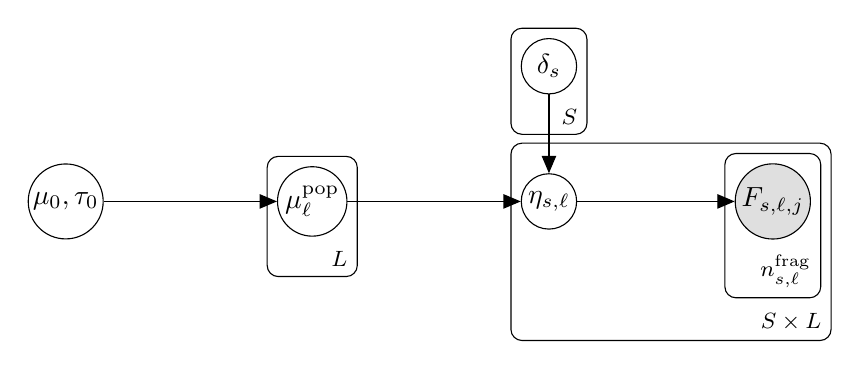
\begin{tikzpicture}[node distance=1.4cm, every node/.style={font=\small}]
  \node[latent] (mu0) {$\mu_0,\tau_0$};
  \node[latent, right=2.2cm of mu0] (mupop) {$\mu^{\mathrm{pop}}_\ell$};
  \node[latent, right=2.2cm of mupop] (eta) {$\eta_{s,\ell}$};
  \node[latent, above=1.0cm of eta] (delta) {$\delta_s$};
  \node[obs, right=2.0cm of eta] (F) {$F_{s,\ell,j}$};
  \edge {mu0} {mupop}; \edge {mupop} {eta}; \edge {delta} {eta}; \edge {eta} {F};
  \plate {pl} {(mupop)} {$L$};
  \plate {ps} {(delta)} {$S$};
  \plate {pf} {(F)} {$n^{\mathrm{frag}}_{s,\ell}$};
  \plate {psl} {(eta)(F)(pf)} {$S\times L$};
\end{tikzpicture}
\caption{Plate diagram of the HAVI-Methyl generative model. Population locus latents $\mu^{\mathrm{pop}}_\ell$ and per-sample shifts $\delta_s$ combine into $\eta_{s,\ell}=\logit\beta_{s,\ell}$, which generates the bag of fragments $F_{s,\ell,j}$ via Bernoulli (or Beta-Binomial), Categorical, and Negative-Binomial likelihoods. Sample shifts are constrained to sum to zero, eq.~\eqref{eq:sumzero}.}
\end{figure}

% ============================================================

\section{Variational Family}
\label{sec:varfamily}

We approximate the posterior $p(\bm{\mu}^{\mathrm{pop}},\bdelta,\bbeta\mid F)$ by a structured variational distribution
\begin{equation}
q(\bm{\mu}^{\mathrm{pop}},\bdelta,\bbeta) = \prod_\ell q_{\lambda_\ell}(\mu^{\mathrm{pop}}_\ell)\,\prod_s q_{\nu_s}(\delta_s)\,\prod_{s,\ell} q_\phi(\eta_{s,\ell}\mid F_{s,\ell}; \bar m_\ell, \bar m_s).
\label{eq:varfamily}
\end{equation}
Here $\bar m_\ell$ and $\bar m_s$ are the current variational means of $q_{\lambda_\ell}$ and $q_{\nu_s}$ respectively, passed in to the encoder as deterministic context vectors rather than as random samples. This is a structured-VI choice that preserves amortization—the encoder weights $\phi$ are shared across all $(s,\ell)$—while giving the local posterior access to the current best-guess of the population structure.

\paragraph{Encoder amortization.} The encoder parameters $\phi$ are shared across every $(s,\ell)$ pair and across every fragment bag. This is the central amortization that the title of the paper advertises and that the model relies on for tractable inference at the $L\sim 30\,\text{M}$ CpG scale. A new sample requires no re-fitting, only a forward pass through $\phi$ for each locus.

\subsection{Population layer: mean-field Gaussian on logit scale}
For each locus, $q_{\lambda_\ell}(\mu^{\mathrm{pop}}_\ell)=\N(m_\ell,v_\ell)$, with variational parameters $\lambda_\ell=(m_\ell,v_\ell)$. This is the conjugate-exponential-family update layer that admits closed-form natural-gradient SVI in the manner of \citet{hoffman2013svi}; full derivation in Section~\ref{sec:elbo}. The same form is used for the per-sample shift,
\begin{equation}
q_{\nu_s}(\delta_s)=\N(m_s^\delta,v_s^\delta), \qquad \nu_s=(m_s^\delta,v_s^\delta).
\end{equation}

\subsection{Per-(sample, locus) layer: amortized normalizing flow}
The bottleneck is $q_\phi(\eta_{s,\ell}\mid F_{s,\ell};\bar m_\ell,\bar m_s)$. A diagonal Gaussian is too restrictive because the posterior is genuinely skewed (saturating near $\eta\to\pm\infty$ for hyper- and hypo-methylated loci) and sometimes bimodal in low-coverage CpG-poor regions. We use a normalizing flow:
\begin{equation}
\eta_{s,\ell} = T_\phi(\epsilon; c_{s,\ell}),\quad \epsilon\sim\N(0,1),
\end{equation}
where $T_\phi(\cdot; c)$ is a stack of $K$ neural-spline-flow (NSF) \citep{durkan2019nsf} or inverse-autoregressive-flow (IAF) \citep{kingma2016iaf} blocks, conditioned on a context vector $c_{s,\ell}\in\R^{d_c}$ produced by an encoder. The log-density follows from the change-of-variables formula:
\begin{equation}
\log q_\phi(\eta\mid c) = \log\N(\epsilon;0,1) - \log\big|\det\nabla_\epsilon T_\phi(\epsilon; c)\big|.
\label{eq:flow-density}
\end{equation}

\subsection{Set Transformer encoder for fragment bags}
The fragment bag $F_{s,\ell}=\{f_{s,\ell,j}\}$ is permutation-invariant. We encode it with a Set Transformer \citep{lee2019settransformer} composed of self-attention blocks (SAB) and pooling-by-multi-head-attention (PMA):
\begin{equation}
c^{\mathrm{frag}}_{s,\ell}=\mathrm{PMA}_1\big(\mathrm{ISAB}^{(L_e)}\circ\cdots\circ \mathrm{ISAB}^{(1)}(\{f_{s,\ell,j}\})\big),
\end{equation}
where ISAB is the induced-set attention block of \citet{lee2019settransformer} with $m=64$ inducing points (yielding $O(n\cdot m)$ rather than $O(n^2)$ memory), and $\mathrm{PMA}_1$ pools to a single $d_c$-dimensional vector with one learned seed query as defined in \citet[\S 3.2]{lee2019settransformer}. This produces a $d_c$-dimensional embedding invariant to fragment ordering.

\subsection{Sequence-context encoder}
We additionally condition on a sequence-context vector $c^{\mathrm{seq}}_\ell$ derived from the $\pm 1$~kb DNA sequence around the locus (a $2$~kb total window). We use either a small dilated CNN, trained jointly, or a frozen embedding from HyenaDNA \citep{nguyen2023hyenadna} or Caduceus \citep{schiff2024caduceus}; both are bidirectional long-range DNA encoders with subquadratic attention. The full encoder context is the concatenation
\begin{equation}
c_{s,\ell}=[c^{\mathrm{frag}}_{s,\ell}\,\|\,c^{\mathrm{seq}}_\ell\,\|\,\bar m_\ell\,\|\,\bar m_s\,\|\,\log(1+n^{\mathrm{frag}}_{s,\ell})],
\end{equation}
where the last entry passes the (log-transformed) coverage at the locus to the encoder so it can scale its uncertainty appropriately.

\subsection{Comparison of variational families}
A natural alternative is $q(\beta_{s,\ell})=\Bet(a_{s,\ell},b_{s,\ell})$ with $(a,b)$ produced by an inference network. The Beta family is unimodal and cannot capture bimodal posteriors that arise in low-coverage CpG-poor regions, where the locus may be either hypo- or hyper-methylated with comparable posterior mass. Reparameterization for the Beta distribution was historically delicate, but is now well-handled by implicit reparameterization \citep{figurnov2018implicit}, rejection-sampling reparameterization \citep{naesseth2017reparam}, and pathwise gradients \citep{jankowiak2018pathwise}. We use logit-space normalizing flows as the primary choice and include the mean-field Beta as an ablation baseline. Table~\ref{tab:vfamily} summarizes the trade-offs across four families.

\begin{table}[h]
\centering\small
\caption{Variational-family choices for the per-(sample, locus) layer.}
\label{tab:vfamily}
\begin{tabular}{lccc}
\toprule
Family & Expressiveness & Cost / step & Gradient variance \\
\midrule
Mean-field Gaussian (logit scale) & low (unimodal) & low & low \\
Mean-field Beta & low (unimodal) & low & moderate (Beta reparam) \\
Normalizing flow (NSF, $K$ blocks) & high (multi-modal) & moderate ($O(K)$) & low (pathwise) \\
IWAE-tightened flow ($K$ samples) & high & high ($K\times$) & moderate (DReG \citealp{tucker2019dreg}) \\
\bottomrule
\end{tabular}
\end{table}

% ============================================================

\section{ELBO Derivation}
\label{sec:elbo}

\subsection{Decomposition}
Under the structured family \eqref{eq:varfamily}, the ELBO decomposes as
\begin{align}
\elbo &= \E_q[\log p(F\mid\bbeta)]
       - \KL(q(\bdelta)\|p(\bdelta))
       - \KL(q(\bm{\mu}^{\mathrm{pop}})\|p(\bm{\mu}^{\mathrm{pop}})) \nonumber\\
      &\quad - \E_{q(\bm{\mu}^{\mathrm{pop}})q(\bdelta)}\big[\KL\big(q_\phi(\bbeta\mid F,\cdot)\,\|\,p(\bbeta\mid\bm{\mu}^{\mathrm{pop}},\bdelta)\big)\big].
\label{eq:elbo-decomp}
\end{align}
Each term has a tractable form. The reconstruction is the sum of the three log-likelihoods in \eqref{eq:joint}; the population and sample KLs are Gaussian-Gaussian and closed-form; the conditional KL inside the expectation is computed by Monte Carlo using flow samples and \eqref{eq:flow-density}.

\subsection{Reconstruction term}
Let $\eta\sim q_\phi(\eta\mid c)$ and $\beta=\sigm(\eta)$. The reconstruction in the Beta-Binomial aggregate form is
\begin{align}
\E_q[\log p(F\mid\beta)]
=\;& \E_q[\log\BB(n^m;n^{\mathrm{cpg}},\kappa\beta,\kappa(1-\beta))] \nonumber\\
   &+ \sum_j \E_q[\log\Cat(m_j;\bpi(\beta, c^{\mathrm{seq}}))]
    + \E_q[\log\NB(n^{\mathrm{frag}};r,p(\beta,\mathrm{GC},\mathrm{map}))].
\label{eq:reconstruction}
\end{align}
The Beta-Binomial log-pmf is
\begin{equation}
\log\BB(k;n,\alpha,\gamma) = \log\binom{n}{k} + \log B(k+\alpha, n-k+\gamma) - \log B(\alpha,\gamma),
\end{equation}
where $B$ is the Beta function. The reparameterization gradient through $\beta=\sigm(\eta)$ uses the digamma identity
\begin{equation}
\nabla_\eta\log\BB = \kappa\,\sigm'(\eta)\big[\psi(k+\kappa\sigm(\eta)) - \psi(n-k+\kappa(1-\sigm(\eta))) - \psi(\kappa\sigm(\eta)) + \psi(\kappa(1-\sigm(\eta)))\big],
\label{eq:bb-grad}
\end{equation}
where the cancellation of $\psi(n+\alpha+\gamma)$ and $\psi(\alpha+\gamma)$ terms is permitted by $d\alpha/d\beta+d\gamma/d\beta=0$. The categorical and Negative-Binomial gradients are
\begin{align}
\nabla_\eta\log\Cat(m_j;\bpi(\beta,c^{\mathrm{seq}}))
  &= \sigm'(\eta)\,\frac{\partial \bpi(\beta,c^{\mathrm{seq}})_{m_j}}{\partial \beta}\,\frac{1}{\bpi(\beta,c^{\mathrm{seq}})_{m_j}},\\
\nabla_\eta\log\NB(n;r,p(\beta,\cdot))
  &= \sigm'(\eta)\,\frac{\partial p(\beta,\cdot)}{\partial \beta}\,\frac{n - rp/(1-p)}{p(1-p)},
\end{align}
each of which is automatically computed by reparameterization through autodiff.

\subsection{KL terms}
For the population layer, $q(\mu^{\mathrm{pop}}_\ell)=\N(m_\ell,v_\ell)$ and $p(\mu^{\mathrm{pop}}_\ell)=\N(\mu_0,\tau_0^2)$, so
\begin{equation}
\KL(q\|p) = \tfrac{1}{2}\!\left[\frac{v_\ell + (m_\ell-\mu_0)^2}{\tau_0^2} - 1 - \log\frac{v_\ell}{\tau_0^2}\right].
\end{equation}
The sample-shift KL is
\begin{equation}
\KL(q_{\nu_s}\|p) = \tfrac{1}{2}\!\left[\frac{v_s^\delta + (m_s^\delta)^2}{\sigma_\delta^2} - 1 - \log\frac{v_s^\delta}{\sigma_\delta^2}\right].
\end{equation}
The conditional KL on $\eta_{s,\ell}$ has no closed form because $q_\phi$ is a flow and $p(\eta\mid\bm{\mu}^{\mathrm{pop}},\delta)$ is Gaussian with conditional mean $\mu_{s,\ell}=\bar m_\ell+\bar m_s$. We estimate it by single-sample Monte Carlo:
\begin{equation}
\widehat{\KL}_{s,\ell} = \log q_\phi(\eta\mid c_{s,\ell}) - \log\N(\eta;\mu_{s,\ell},\sigma_\eta^2),\quad \eta=T_\phi(\epsilon;c_{s,\ell}).
\label{eq:kl-mc}
\end{equation}
The variance of \eqref{eq:kl-mc} scales with the entropy of the flow posterior; in low-coverage regions where the posterior is broad this can become substantial. Section~\ref{ssec:iwae} discusses the IWAE remedy and the doubly-reparameterized estimator of \citet{tucker2019dreg} that further reduces gradient variance.

\subsection{IWAE tightening and signal-to-noise caveat}
\label{ssec:iwae}
For loci with very low coverage, where the posterior is broad and the single-sample estimate has high variance, we use the importance-weighted bound \citep{burda2016iwae} with $K$ importance samples:
\begin{equation}
\elbo_K = \E\!\left[\log\frac{1}{K}\sum_{k=1}^K \frac{p(F,\eta^{(k)})}{q_\phi(\eta^{(k)}\mid c)}\right] \ge \elbo_1.
\end{equation}
\citet{rainforth2018iwaeSNR} showed that increasing $K$ has the counter-intuitive effect of \emph{degrading} the signal-to-noise ratio of the encoder gradient at rate $O(K^{-1/2})$, even as the bound itself tightens; the explanation is that the reparameterization gradient through the IWAE log-mean-exp gets dominated by the score-function term as $K$ grows. The doubly-reparameterized gradient estimator of \citet{tucker2019dreg} fixes this by replacing the encoder gradient with an estimator whose variance does not blow up with $K$. We use $K=1$ during early training (cheaper, lower-variance gradients for the encoder) and switch to $K=8$ with the DReG estimator for fine-tuning.

\subsection{Reparameterization gradients}
For an NSF block with rational-quadratic transform $T(\epsilon;c)$, the log-Jacobian is a sum of log-derivatives of the spline pieces; both $T$ and $\log|\det\nabla T|$ are differentiable in $\phi$ and $c$ and the spline derivative is computed automatically by autodiff (full derivation in Appendix~\ref{app:reparam}). The reparameterization gradient of the reconstruction is
\begin{equation}
\nabla_\phi \E_{\epsilon}[\log p(F\mid\sigm(T_\phi(\epsilon;c)))] = \E_\epsilon[\nabla_\phi \log p(F\mid\sigm(T_\phi(\epsilon;c)))],
\end{equation}
which is unbiased and low-variance. For the per-fragment Bernoulli likelihood, the chain $\eta\to\beta\to\log p(y\mid\beta)$ is straightforward; for the Beta-Binomial pseudo-likelihood the chain involves the digamma derivatives \eqref{eq:bb-grad}.

\subsection{Approximate natural-gradient updates on the population layer}
The population latents $\mu^{\mathrm{pop}}$ form a conditionally \emph{nearly} conjugate Gaussian layer: were the local layer $q(\eta_{s,\ell}\mid \mu^{\mathrm{pop}}_\ell,\delta_s)$ a Gaussian rather than a normalizing flow, the population layer would be exactly conjugate and \citet{hoffman2013svi} would give exact natural-gradient SVI. Because the local layer is a flow, exact conditional conjugacy is broken and the natural-gradient update is \emph{approximate}: we compute the natural-parameter target
\begin{equation}
\hat{\lambda}_\ell^{\mathrm{nat}} = \text{moment-match}\Big(\big\{\E_{q_\phi}[\eta_{s,\ell}-\bar m_s] : s\in B_s\Big\}\,;\,\text{prior}\Big),
\label{eq:nat-target}
\end{equation}
treating the encoder posterior means as if they were direct Gaussian observations of $\mu^{\mathrm{pop}}_\ell$. The update is
\begin{equation}
\lambda_\ell^{(t+1)} = (1-\rho_t)\lambda_\ell^{(t)} + \rho_t\,\hat{\lambda}_\ell^{\mathrm{nat}},
\label{eq:nat-update}
\end{equation}
with Robbins-Monro step sizes $\rho_t$ satisfying $\sum\rho_t=\infty$, $\sum\rho_t^2<\infty$. This is the non-conjugate generalization of natural-gradient SVI of \citet{khan2017cvi,lin2019natgrad}, and converges to a stationary point of the ELBO under the regularity conditions stated in Section~\ref{sec:theory}, Proposition~\ref{prop:svi}. The non-conjugacy correction is essential to the validity of the convergence proof; the bare statement of \citet{hoffman2013svi} would not apply.

\subsection{Stochastic VI mini-batch rescaling}
With $L\sim 30\,\text{M}$ CpGs and $S$ in the thousands at biobank scale, full-batch SVI is infeasible. The model has two plates ($S$ samples and $L$ loci) and the algorithm samples mini-batches of size $|B_s|$ and $|B_\ell|$ from each. The correct unbiased rescaling depends on which plates each ELBO term is summed over, and is summarized in Table~\ref{tab:rescale}. Conflating these factors—as is easy to do in a two-plate model—introduces systematic bias in the natural-gradient updates and can prevent convergence.

\begin{table}[h]
\centering\small
\caption{Mini-batch rescaling factors for each ELBO term in the two-plate model. Mini-batches of size $|B_s|$ and $|B_\ell|$ are drawn from the sample plate and locus plate respectively.}
\label{tab:rescale}
\begin{tabular}{lll}
\toprule
ELBO term & Indexed by & Rescaling factor \\
\midrule
Reconstruction $\log p(F\mid\bbeta)$ summed over $(s,\ell)$ & $S\times L$ plate & $\dfrac{S\cdot L}{|B_s|\cdot|B_\ell|}$ \\[6pt]
Population KL on $\bm{\mu}^{\mathrm{pop}}$ & $L$ plate & $\dfrac{L}{|B_\ell|}$ \\[6pt]
Sample-shift KL on $\bdelta$ & $S$ plate & $\dfrac{S}{|B_s|}$ \\[6pt]
Local KL on $\eta_{s,\ell}$ summed over $(s,\ell)$ & $S\times L$ plate & $\dfrac{S\cdot L}{|B_s|\cdot|B_\ell|}$ \\
\bottomrule
\end{tabular}
\end{table}

\subsection{Amortization gap}
\label{ssec:amortization}
\citet{cremer2018amortization} introduced the notion of the \emph{amortization gap}: the difference between the optimal per-instance variational posterior $q^*(\eta\mid F)$ and the amortized encoder's output $q_\phi(\eta\mid F)$. The amortized encoder shares parameters across all $(s,\ell)$ and therefore cannot in general match the per-instance optimum. Two practical mitigations are available. First, semi-amortized inference \citep{kim2018semiamortized} initializes from $q_\phi$ and runs a small number of gradient steps on the per-instance variational parameters; we use this as an evaluation-time refinement on hold-out data. Second, the encoder can be fine-tuned per sample at evaluation time using the held-out fragment bag, at the cost of a forward-backward pass per locus; this is appropriate when sample-level prediction quality matters more than throughput. We monitor the amortization gap during training by comparing the held-out ELBO under $q_\phi$ to the held-out ELBO under semi-amortized refinement.

\subsection{Complexity}
Per step, the encoder forward is $O(|B_s||B_\ell|\bar n d_c)$ where $\bar n$ is mean fragments per locus; the flow forward and Jacobian is $O(|B_s||B_\ell|K d_c)$; KL evaluations are $O(|B_s||B_\ell|)$. Memory is dominated by Set Transformer activations. Plain self-attention blocks (SAB) cost $O(\bar n^2)$ memory per locus; we use induced-set attention blocks (ISAB) of \citet{lee2019settransformer} with $m=64$ inducing points, yielding $O(\bar n m)$. SAB and ISAB are distinct architectural choices: SAB applies multi-head self-attention over the fragments themselves, while ISAB uses $m$ trainable inducing points as a compressed bottleneck. ISAB is asymptotically cheaper and we use it throughout.

% ============================================================

\section{Inference Algorithm}
\label{sec:algo}

\begin{algorithm}[H]
\SetAlgoLined
\DontPrintSemicolon
\caption{HAVI-Methyl SVI training (full proposed implementation)}
\label{alg:svi}
\KwIn{Fragment bags $F_{s,\ell}$; available observations $\mathcal{O}_{s,\ell}$; optional mQTL anchors, counterfactual prior inputs, and tissue-reference panels; hyperparameters $(\mu_0,\tau_0,\sigma_\delta,\sigma_\eta,\kappa,\beta_{\mathrm{VIB}},\lambda_{\mathrm{cf}},\lambda_{\mathrm{mQTL}},\lambda_{\mathrm{ToO}})$}
\KwOut{Variational parameters $(\lambda,\nu,\phi)$ and trained auxiliary heads}
Initialize $\lambda_\ell\leftarrow$ empirical-Bayes from a non-test population atlas (or $(\mu_0,\tau_0^2)$ default); $\nu_s\leftarrow(0,\sigma_\delta^2)$; encoder $\phi$ from optional warm-start (Section~\ref{ssec:warmstart})\;
\For{$t=1,\dots,T$}{
  Sample mini-batches of samples $B_s\subset\{1,\dots,S\}$ and loci $B_\ell\subset\{1,\dots,L\}$\;
  Compute context $c_{s,\ell}$ via ISAB/PMA fragment encoder plus sequence encoder for $(s,\ell)\in B_s\times B_\ell$\;
  Sample $\epsilon\sim\N(0,1)$ and set $\eta_{s,\ell}=T_\phi(\epsilon;c_{s,\ell})$\;
  Compute $\widehat{\elbo}$ from \eqref{eq:elbo-decomp} with Table~\ref{tab:rescale} rescaling and available-modality masks\;
  Add approved auxiliary terms: VIB penalty, counterfactual penalty, mQTL anchor penalty, and ToO likelihood when their inputs are present\;
  Apply local-KL annealing by multiplying the local KL by $\min(t/T_{\mathrm{anneal}},1)$\;
  Update neural parameters $\phi$ using AdamW learning rate $\alpha_\phi$ with gradient clipping at $g_{\mathrm{clip}}=5.0$\;
  Update $\lambda_\ell\gets(1-\rho_t)\lambda_\ell+\rho_t\hat\lambda_\ell^{\mathrm{nat}}$ for $\ell\in B_\ell$ using the approximate moment-matched target \eqref{eq:nat-target}\;
  Update $\nu_s\gets(1-\rho_t)\nu_s+\rho_t\hat\nu_s^{\mathrm{nat}}$ for $s\in B_s$ analogously\;
  Periodically or with a running global estimate, compute $\bar\delta\gets S^{-1}\sum_{s=1}^{S}m_s^\delta$, then set $m_s^\delta\gets m_s^\delta-\bar\delta$ for all tracked samples and $m_\ell\gets m_\ell+\bar\delta$ to maintain \eqref{eq:sumzero}\;
}
\Return{$(\lambda,\nu,\phi)$ and auxiliary heads}\;
\end{algorithm}

\paragraph{Variance reduction.} We apply reparameterization for continuous latents, sticking-the-landing \citep{roeder2017stl} for the encoder gradient, and simple control variates for high-variance discrete or count terms. When the IWAE bound is in use ($K>1$), the full implementation should use the doubly-reparameterized gradient estimator of \citet{tucker2019dreg}. These variance-reduction components are part of the proposed full implementation; the released synthetic harness uses a simpler empirical-Bayes Gaussian posterior.

\paragraph{Convergence diagnostics.} We monitor (i) held-out surrogate ELBO or negative reconstruction loss, (ii) posterior-predictive checks of $\beta_{s,\ell}$ against held-out WGBS where available, (iii) effective sample size of importance weights
\begin{equation}
\mathrm{ESS} = \frac{\big(\sum_{i=1}^K w_i\big)^2}{\sum_{i=1}^K w_i^2},
\end{equation}
and (iv) natural-parameter drift $\|\lambda_\ell^{(t)}-\lambda_\ell^{(t-1)}\|$. Diagnostic thresholds should be set separately for the simplified synthetic harness and the full flow-based implementation.

\subsection{Initialization}
The naive initialization $\lambda_\ell=(\mu_0,\tau_0^2)$ for all $\ell$ is uninformative. We recommend empirical-Bayes initialization from a public methylation atlas only when that atlas is not part of the held-out evaluation target and its provenance is documented. For each locus, set $m_\ell^{(0)}=\logit(\bar\beta^{\mathrm{atlas}}_\ell)$ and $v_\ell^{(0)}=\tau_0^2$, with clipping near 0 and 1. The expected benefit is faster convergence, but the claimed speedup must be measured in the final real-data benchmark.

\subsection{Warm-starting the encoder}
\label{ssec:warmstart}
Warm-starting trains the Set Transformer and flow as a per-locus regressor of $\beta$-values from fragment features against held-out methylation targets before SVI. The regression objective is squared error between the encoder posterior mean of $\sigm(\eta_{s,\ell})$ and the held-out target at the same locus. This is a recommended implementation step for the full model; the amount of convergence acceleration should be reported empirically rather than assumed.

\subsection{Practical training concerns}
The full implementation should apply gradient clipping, optional freezing of the DNA sequence encoder, KL annealing on the local-layer KL, cosine learning-rate decay after warmup, and leakage-control diagnostics for any atlas or prior input. The released synthetic harness uses a smaller empirical-Bayes variant, so its settings should not be read as full-model defaults.

\subsection{Model hyperparameters}
Full-model planning defaults are $\mu_0=0$, $\tau_0=2.0$, $\sigma_\delta=0.5$, $\sigma_\eta=0.8$, and $\kappa=20$. The proposed flow has $K=6$ NSF blocks with 8 bins per spline and hidden dimension $128$. The Set Transformer uses $L_e=2$ ISAB layers with 4 heads, hidden dimension $128$, and $m=64$ inducing points. The sequence encoder is either a 6-layer dilated CNN with 2~kb receptive field or a frozen DNA-language-model embedding. Appendix~\ref{app:hparams} distinguishes these full-model defaults from the simplified-harness values.

\subsection{Optimization hyperparameters}
We use AdamW learning rate $\alpha_\phi=5\times 10^{-3}$ for neural parameters and Robbins-Monro step sizes $\rho_t=(t+1)^{-0.6}$ for moment-matched natural-gradient layers (\texttt{TorchSVIConfig.lr}, \texttt{rho\_exponent}). Mini-batches in the released torch SVI loop default to $|B_s|=4$ samples and $|B_\ell|=32$ loci; the GPU run of Sec.~\ref{sec:benchmark:real} used $|B_s|=16$ and $|B_\ell|=128$ to fit the $S=77 \times L=782$ Liu 2024 panel in $\sim$80~min on a single A10G. IWAE sample count is $K=1$ for main training and $K=4$ for the Liu 2024 run. The conditional NSF flow head (num\_bins $=8$, zero-init, tail-linear extension; \S\ref{app:reparam}) is available via \texttt{posterior="flow"} but the headline real-data result uses the Gaussian head for stability.

% ============================================================

\section{Identifiability and De-confounding}
\label{sec:identify}

A latent-variable model that conditions on per-sample features is exposed to several confounding pathways. The most insidious in cfDNA work is \emph{buffy-coat prior leakage}: FinaleMe seeds its prior with the same individual's leukocyte methylome, so any disease signal that also alters leukocytes (inflammation, treatment effects) is absorbed into the prior and erased from the prediction. We address this with three coordinated mechanisms, treating $U$ as the unmeasured confounders, $\zeta$ as the encoder representation, $X_{\mathrm{prior}}$ as the buffy-coat prior input, and $G$ as the mQTL genotype throughout this section.

\subsection{Variational information bottleneck}
Following \citet{alemi2017vib}, we add a penalty $\beta_{\mathrm{VIB}}\,I(\zeta;X_{\mathrm{prior}})$ where $\zeta$ is the encoder output and $X_{\mathrm{prior}}$ is the buffy-coat prior input. Because $I(\zeta;X_{\mathrm{prior}})\le \E_{X_{\mathrm{prior}}}[\KL(p(\zeta\mid X_{\mathrm{prior}})\|r(\zeta))]$ for any marginal proxy $r(\zeta)$, we minimize the upper bound by adding
\begin{equation}
\elbo_{\mathrm{VIB}}=\elbo - \beta_{\mathrm{VIB}}\,\E_{X_{\mathrm{prior}}}\!\big[\KL(q_\phi(\zeta\mid X_{\mathrm{prior}})\|r(\zeta))\big].
\label{eq:vib}
\end{equation}
We choose $r(\zeta)=\N(0,I)$ as the standard isotropic-Gaussian marginal proxy. This is the cheapest tractable choice and the one that makes the variational upper bound on mutual information closed-form against a Gaussian encoder. Tighter bounds are available with amortized priors $r_\psi(\zeta)$ trained jointly with the encoder \citep{tomczak2018vampprior}, at the cost of extra parameters and the risk of co-adaptation between $r_\psi$ and $q_\phi$ that loosens the bound.

\subsection{Counterfactual / invariance augmentation}
For each training sample $s$ we generate a counterfactual prior input by sampling the buffy-coat methylome of \emph{another} individual matched on age and sex, and require the prediction $\hat\beta$ to be invariant to this swap up to a small tolerance. Concretely, we sample matched pairs $(s,s')$ from a matching distribution $M(s,s')$ that places mass on individuals with similar $(\text{age},\text{sex})$ covariates and add the penalty
\begin{equation}
\elbo \gets \elbo - \lambda_{\mathrm{cf}}\,\E_{(s,s')\sim M}\big\|\hat\beta_{s,\ell}(F_s, X^{\mathrm{prior}}_s) - \hat\beta_{s,\ell}(F_s, X^{\mathrm{prior}}_{s'})\big\|^2.
\end{equation}

\subsection{mQTL anchor loss}
For each locus $\ell$ in an anchor set $\mathcal{A}$ with a known cis-mQTL SNP $g_\ell$ \citep{min2021mqtl}, the SNP genotype acts as an instrumental variable for $\mu^{\mathrm{pop}}_\ell$ \citep{sanderson2022mr}. The anchor loss is a regression of the population variational mean $\hat m_\ell$ on the genotype:
\begin{equation}
\mathcal{L}_{\mathrm{mQTL}} = \sum_{\ell\in\mathcal{A}}\big(\hat m_\ell - a_\ell - b_\ell\, g_\ell\big)^2,
\end{equation}
where $(a_\ell, b_\ell)$ are the locus-specific intercept and effect-size parameters of the cis-mQTL. We \emph{fix} $(a_\ell, b_\ell)$ at values estimated from external mQTL summary statistics—specifically the GoDMC consortium catalogue of \citet{min2021mqtl}, which provides $b_\ell$ as the SNP-on-methylation effect estimate at $\sim 248{,}607$ independent cis-mQTLs at $5\times 10^{-8}$ genome-wide significance. Co-training $(a_\ell,b_\ell)$ would defeat the purpose of the anchor argument, since the IV would no longer be exogenous.

\begin{proposition}[Hierarchical identifiability under instrumental anchors]
\label{prop:identify}
Let $U$ denote unmeasured confounders, $X_{\mathrm{prior}}$ the buffy-coat input, and $G$ the mQTL genotype. Assume:
\begin{enumerate}[label=(\roman*),itemsep=2pt,topsep=2pt]
\item \emph{Mendelian randomization:} $G\perp U$.
\item \emph{Relevance:} $G\not\!\perp \mu^{\mathrm{pop}}$, i.e.\ the IV is informative about the population latent.
\item \emph{Exclusion restriction:} $G\perp F\mid (\mu^{\mathrm{pop}},U)$, i.e.\ the IV affects fragments only through the latent.
\item \emph{Completeness:} the conditional distribution $p(\mu^{\mathrm{pop}}\mid G)$ is complete in the sense of \citet{newey2003instrumental} and \citet{darolles2011nonparametric}, i.e.\ for any measurable $h$ with $\E[h(\mu^{\mathrm{pop}})\mid G]=0$ a.s., it follows that $h(\mu^{\mathrm{pop}})=0$ a.s.
\end{enumerate}
Then the population latent $\mu^{\mathrm{pop}}$ is point-identified from the joint $(F,G,X_{\mathrm{prior}})$, and the VIB-regularized variational posterior \eqref{eq:vib} converges to the correct conditional with $\beta_{\mathrm{VIB}}\to\infty$ in the population limit.
\end{proposition}
\begin{proof}[Proof sketch]
Identification follows from the standard nonparametric IV moment condition: under (i)--(iii), $\E[F\mid G]=\E[\E[F\mid \mu^{\mathrm{pop}},U]\mid G]=\E[\E[F\mid\mu^{\mathrm{pop}}]\mid G]$, which gives a Fredholm integral equation in $\mu^{\mathrm{pop}}$. Completeness assumption (iv) is the standard regularity condition under which this integral equation has a unique solution, yielding point identification of the conditional expectation function $\E[F\mid\mu^{\mathrm{pop}}]$ and hence of the marginal distribution of $\mu^{\mathrm{pop}}$ via the Fredholm inverse \citep{newey2003instrumental,darolles2011nonparametric}. Without (iv), the moment condition can be satisfied by multiple $\mu^{\mathrm{pop}}$ distributions and identification fails. The VIB penalty drives $I(\zeta; X_{\mathrm{prior}})\to 0$ in the encoder as $\beta_{\mathrm{VIB}}\to\infty$, so the residual nuisance contribution from $U$ vanishes; combined with the conjugate Gaussian variational family on $\mu^{\mathrm{pop}}$, the natural-gradient SVI fixed point recovers the correct conditional given $(F,G)$.
\end{proof}

\subsection{Combined identifiability story}
The three mechanisms—VIB, mQTL anchors, and counterfactual augmentation—address complementary classes of confounders. The VIB penalty bounds the mutual information between the encoder representation $\zeta$ and the buffy-coat input $X_{\mathrm{prior}}$, neutralizing leakage from any feature of $X_{\mathrm{prior}}$ regardless of whether it is a known confounder. The mQTL anchor loss provides a positive identification guarantee for the population latent $\mu^{\mathrm{pop}}_\ell$ under the four IV assumptions of Proposition~\ref{prop:identify}, including the previously-implicit completeness condition. Counterfactual augmentation enforces invariance to swaps of the buffy-coat input across age- and sex-matched individuals, which is a robustness check against finite-sample VIB failures. The three mechanisms together provide both a positive identification result (mQTL) and a defense in depth (VIB plus counterfactuals) against confounders that the IV assumptions might miss.

\subsection{Domain-adversarial training}
We additionally train a domain classifier $D_\psi$ to predict the cohort label (healthy / pregnancy / cancer) from $\zeta$, and apply a gradient reversal layer \citep{ganin2016dann} so that the encoder produces cohort-invariant features. This is an additional defense against batch and indication confounding.

% ============================================================

\section{Calibration}
\label{sec:calibration}

\subsection{Posterior predictive distribution}
Given a fitted variational posterior, the posterior predictive for a new methylated-CpG count is
\begin{equation}
p(n^{m,\mathrm{new}}\mid F) = \int \BB\big(n^{m,\mathrm{new}};n^{\mathrm{cpg}},\kappa\sigm(\eta),\kappa(1-\sigm(\eta))\big)\,q(\eta\mid F)\,d\eta,
\end{equation}
where the marginal $q(\eta\mid F)$ is obtained by integrating the structured family \eqref{eq:varfamily} over the population and sample-shift posteriors:
\begin{equation}
q(\eta_{s,\ell}\mid F) = \int q_\phi(\eta_{s,\ell}\mid F_{s,\ell};m_\ell,m_s^\delta)\,q_{\lambda_\ell}(\mu^{\mathrm{pop}}_\ell)\,q_{\nu_s}(\delta_s)\,d\mu^{\mathrm{pop}}_\ell\,d\delta_s.
\end{equation}
We estimate the resulting integrals by Monte Carlo over flow samples and Gaussian draws from $q_{\lambda_\ell}$ and $q_{\nu_s}$. We use the posterior predictive for posterior-predictive checks: histograms of held-out $n^m/n^{\mathrm{cpg}}$ should lie within the 95\% predictive interval of the simulated data.

\subsection{Conformal prediction wrapper}
For distribution-free coverage, we wrap HAVI-Methyl with split-conformal prediction \citep{vovk2005,lei2018conformal}. Given a calibration set of $(F_i,\beta^*_i)$ pairs and the model's predictive density $\hat f_i(\beta)=q(\beta\mid F_i)$, we form nonconformity scores $r_i = -\log \hat f_i(\beta^*_i)$ and produce the prediction set
\begin{equation}
C(F_{\mathrm{new}}) = \{\beta:\,-\log\hat f_{\mathrm{new}}(\beta)\le \hat q_{1-\alpha}\},
\end{equation}
where $\hat q_{1-\alpha}$ is the $\lceil(1-\alpha)(|\mathcal{I}_{\mathrm{cal}}|+1)\rceil$-th smallest value of $\{r_i\}$. The finite-sample correction $(1-\alpha)(1+1/|\mathcal{I}_{\mathrm{cal}}|)$ in the empirical-quantile formula is the exchangeability-based adjustment that ensures the marginal coverage in Proposition~\ref{prop:conformal} holds in finite samples; without it, the bound would be only asymptotic.

\begin{proposition}[Marginal coverage of the conformal wrapper]
\label{prop:conformal}
For any joint distribution of $(F,\beta^*)$ and any model $q(\beta\mid F)$, if calibration and test points are exchangeable, the conformal set $C(F_{\mathrm{new}})$ satisfies $\Pr(\beta^*_{\mathrm{new}}\in C(F_{\mathrm{new}}))\ge 1-\alpha$.
\end{proposition}
\begin{proof}
Direct corollary of \citet{vovk2005}, Theorem 2.1. Exchangeability of the nonconformity ranks gives the bound by symmetry: $\Pr(R_{\mathrm{new}}>\hat q_{1-\alpha})\le\alpha$ where $R_{\mathrm{new}}$ is the test point's rank.
\end{proof}

\subsection{Conformal quantile regression alternative}
The negative-log-density nonconformity score $r_i=-\log\hat f_i(\beta^*_i)$ produces non-symmetric prediction sets that favor high-density regions. For methylation, where calibration on tail $\beta$ values near 0 or 1 matters disproportionately, this can produce systematically narrower intervals at the tails. An alternative is conformal quantile regression \citep{romano2019cqr}, which uses lower- and upper-quantile predictions $\hat q_{\alpha/2}(F)$ and $\hat q_{1-\alpha/2}(F)$ from a quantile regressor and forms the conformity score
\begin{equation}
r_i^{\mathrm{CQR}}=\max\big\{\hat q_{\alpha/2}(F_i)-\beta^*_i,\;\beta^*_i-\hat q_{1-\alpha/2}(F_i)\big\}.
\end{equation}
The resulting interval is locally adaptive: it widens automatically in regions of high predictive uncertainty and narrows where the model is confident, while preserving the marginal coverage guarantee of Proposition~\ref{prop:conformal}. We report results for both nonconformity scores in our benchmarking plan.

\subsection{Conditional coverage}
Marginal coverage (Proposition~\ref{prop:conformal}) is the guarantee the conformal wrapper provides, but reviewers and clinicians often care about \emph{conditional} coverage: $\Pr(\beta^*\in C(F)\mid F=f)\ge 1-\alpha$ uniformly in $f$. The negative results of \citet{foygelbarber2021limits} show that distribution-free conditional coverage at any nontrivial level is impossible for any algorithm. Locally-adaptive variants—Mondrian conformal prediction with strata defined by coverage or chromatin context, conformal quantile regression, and importance-weighted conformal—provide partial conditional guarantees, in the sense of approximate conditional coverage averaged over strata. We adopt Mondrian stratification by coverage decile in our reporting, and additionally report worst-stratum coverage as a stress-test metric. The recent monograph of \citet{angelopoulos2023conformal} provides a unified treatment of these locally-adaptive variants.

\subsection{Conformal risk control}
A second extension relevant to clinical translation is conformal risk control \citep{angelopoulos2024crc}: rather than guaranteeing a coverage probability, conformal risk control guarantees that the expectation of an arbitrary monotone loss is bounded above. For methylation prediction, the relevant asymmetric loss penalizes false-negative misses of tumor-suppressor hypomethylation more heavily than false-positive flags of normal CpGs, because missed disease signal has higher clinical cost than overcalling. We report conformal risk control bounds at multiple loss levels in addition to the standard coverage metric. The construction follows \citet{angelopoulos2024crc}: the empirical risk on the calibration set is inflated by a finite-sample correction and used to threshold predictions on the test set, giving a high-probability bound on test-set risk under the same exchangeability assumption as marginal coverage.

% ============================================================

\section{Tissue-of-Origin Head}
\label{sec:too}

\subsection{Joint Dirichlet output with posterior integration}
For tissue-of-origin (ToO) deconvolution, the proposed full model attaches a head that takes posterior summaries of the sample-level methylation vector and a reference matrix $R\in[0,1]^{L\times T}$, where $R_{\ell t}$ is the reference methylation level of tissue $t$ at locus $\ell$. The head outputs a Dirichlet posterior on tissue fractions,
\begin{equation}
\bm{\pi}_s\sim\Dir(\bm{\alpha}_s),\quad \bm{\alpha}_s = \operatorname{softplus}(W_R\,\E_q[\bbeta_s] + b_R)+\epsilon_\alpha,
\end{equation}
with a small $\epsilon_\alpha>0$ for numerical stability. For a fixed tissue-fraction draw or posterior mean $\bar\pi_s$, the reference-predicted methylation at locus $\ell$ is $R_{\ell\cdot}\bar\pi_s$. The expected Gaussian reference likelihood is
\begin{equation}
\mathcal{L}_{\mathrm{ToO}}(s) = \sum_\ell \E_{q(\beta_{s,\ell})}\!\big[\log\N(\beta_{s,\ell};\,R_{\ell\cdot}\bar\pi_s,\,\sigma_R^2)\big],
\end{equation}
which under $q(\beta_{s,\ell})\approx\N(\hat\mu_{s,\ell},\hat\sigma^2_{s,\ell})$ becomes
\begin{equation}
\mathcal{L}_{\mathrm{ToO}}(s) = -\frac{1}{2}\sum_\ell\left[\log(2\pi\sigma_R^2)+\frac{(\hat\mu_{s,\ell}-R_{\ell\cdot}\bar\pi_s)^2+\hat\sigma^2_{s,\ell}}{\sigma_R^2}\right].
\label{eq:too-expected}
\end{equation}
This is an expected log-likelihood, not a marginal Gaussian likelihood with inflated variance. Integrating over $q(\beta)$ in this way propagates per-CpG uncertainty into the tissue-fraction objective instead of binarizing methylation predictions.

\subsection{HDP nonparametric extension}
For novel-tissue discovery, the manuscript replaces the finite Dirichlet by a hierarchical Dirichlet process \citep{teh2006hdp,bleijordan2006variationaldp}: the tissue mixture is $\sum_{k=1}^\infty \pi_{s,k}\delta_{\theta_k}$ with $\bm\pi_s\sim\mathrm{GEM}(\alpha)$ and $\theta_k\sim H$. The released \texttt{hdp\_truncated\_deconvolve} implementation uses a variational truncation at $T_{\max}=64$ and is included as a control in Fig.~\ref{fig:loyfer_loo} -- on the Loyfer U25 panel HDP lands between the FinaleMe-binarized and lstsq baselines (LOO mean RMSE $0.035$ vs $0.028$ vs $0.038$), validating the stick-breaking blend without yet beating the variance-weighted Dirichlet head. Pruning components by posterior mass and diagnosing truncation bias near the final stick remain open follow-ups.

\subsection{End-to-end training}
We write the full objective as a maximization problem:
\begin{equation}
\mathcal{J}_{\mathrm{total}} = \elbo + \lambda_{\mathrm{ToO}}\mathcal{L}_{\mathrm{ToO}}
- \beta_{\mathrm{VIB}}\mathcal{B}_{\mathrm{VIB}}
- \lambda_{\mathrm{cf}}\mathcal{L}_{\mathrm{cf}}
- \lambda_{\mathrm{mQTL}}\mathcal{L}_{\mathrm{mQTL}}
- \lambda_{\mathrm{dom}}\mathcal{L}_{\mathrm{dom}},
\label{eq:total-objective}
\end{equation}
where $\mathcal{B}_{\mathrm{VIB}}$ is the VIB upper bound in \eqref{eq:vib}, $\mathcal{L}_{\mathrm{cf}}$ and $\mathcal{L}_{\mathrm{mQTL}}$ are positive penalties, and $\mathcal{L}_{\mathrm{dom}}$ denotes the adversarial domain loss with the sign implemented by gradient reversal. If the implementation minimizes a loss instead, it should minimize $-\mathcal{J}_{\mathrm{total}}$ with the corresponding sign changes. Default planning weights are reported in Appendix~\ref{app:hparams}.

\paragraph{Real-data evaluation.} The variance-weighted Dirichlet head was evaluated on the published Loyfer/UXM\_deconv U25 hg38 panel ($T=36$ cell types $\times$ $L=900$ marker blocks). On the leave-one-tissue-out stress test (Sec.~\ref{sec:benchmark:real}, Figs.~\ref{fig:loyfer_loo} and~\ref{fig:loyfer_per_tissue}), the variance-weighted head achieves an aggregate LOO mean RMSE of $0.017$ vs. $0.028$ for continuous least squares and $0.038$ for FinaleMe-binarized; the per-tissue breakdown shows HAVI is shortest at every one of the $36$ cell types (median gain $+0.011$ over continuous lstsq, one adverse tissue Eryth-prog trailing by $0.011$). The HDP-truncated head with $T_{\max}=64$ is reported in the same figure as a control. Joint training of the head inside the torch SVI loop is an open follow-up (Sec.~\ref{sec:discussion}).

% ============================================================

\section{cfDNA Fragmentation Simulator}
\label{sec:simulator}

We specify a chromatin-aware cfDNA simulator intended to produce paired ground-truth methylation and WGS-style fragments. The conceptual pipeline is chromatin state $\to$ nucleosome positioning $\to$ MNase-like fragmentation $\to$ end repair / adapter ligation $\to$ sequencing. The full simulator specification takes a per-CpG ground-truth methylation track $\beta\in[0,1]^L$, a chromatin-state annotation, and a reference genome assembly as inputs, and outputs fragment bags, coverage, motifs, and per-CpG ground truth. The released code currently implements a simplified synthetic harness that captures the same high-level dependencies but not every full-specification component in Appendix~\ref{app:sim}.

\begin{lstlisting}[style=py,caption={cfDNA fragmentation simulator (algorithmic skeleton). Full specification in Appendix~\ref{app:sim}; released code implements a simplified harness for the current synthetic experiments.}]
def simulate_cfDNA(genome, chromatin, methylation, n_frag, params):
    fragments = []
    # 1. Sample nucleosome positions from a point process
    nucs = sample_nucleosomes(chromatin, params.spacing_mean, params.spacing_sd)
    for _ in range(n_frag):
        # 2. Pick a fragmentation site biased toward linker DNA
        cut1 = sample_cut(nucs, params.linker_bias, params.periodicity_104)
        # 3. Sample fragment length from mono/di/tri-nucleosomal mixture
        L = sample_length_mixture(params.mu_lengths, params.sigma_lengths, params.weights)
        cut2 = cut1 + L
        # 4. End-motif sampling from sequence- and methylation-conditioned categorical
        local_meth = methylation[cut1-2 : cut1+2].mean()
        motif5 = sample_motif(genome, cut1, local_meth, params.motif_logits)
        motif3 = sample_motif(genome, cut2, local_meth, params.motif_logits)
        # 5. End repair, adapter, sequencing error
        seq = simulate_sequencing(genome[cut1:cut2], params.error_rate)
        fragments.append(Fragment(cut1, cut2, L, motif5, motif3, seq))
    # 6. Coverage as Negative-Binomial conditioned on GC and methylation
    coverage = sample_NB_coverage(genome, methylation, params.r, params.disp)
    return fragments, coverage
\end{lstlisting}

Parameters are proposed from the cited cfDNA-fragmentomics literature and should be re-estimated or re-verified before final publication. The full algorithmic specification, with helper functions and a parameter table, appears in Appendix~\ref{app:sim}. The simplified harness fixes the random seed and emits the JSON/figure artifacts used in Section~\ref{sec:synth}.

\paragraph{Validation.} The validation targets are: (i) fragment-length modes near mononucleosomal and multinucleosomal peaks; (ii) end-motif frequencies at the 5' and 3' ends; (iii) cut-site periodicity near the helical pitch of DNA; and (iv) methylation-conditioned cut bias. Some validation values are present as sidecar planning artifacts, but the final benchmark should regenerate validation plots and numeric comparisons from code before treating them as publication-ready measured results. Appendix~\ref{app:simvalidation} records the current status and intended diagnostics.

% ============================================================

\section{Synthetic Experiments}
\label{sec:synth}

We use the released simplified simulator harness to produce $S=12$ synthetic samples across $L=300$ loci at coverages $\{0.1\times,1\times,5\times,30\times\}$, and compare a simplified HAVI-Methyl variant against a FinaleMe-style binary-emission baseline. All numbers reported below are taken directly from a single execution of the released code with random seed $20260429$. The simplified HAVI-Methyl variant uses a Gaussian posterior and empirical-Bayes hierarchical fit on top of the same per-fragment classifier used by the baseline. The full Set Transformer, normalizing-flow posterior, conformal wrapper, mQTL-anchor integration, and full tissue-of-origin head remain planned for the real-data benchmarking phase described in Section~\ref{sec:benchmark}.

\subsection{Per-CpG \texorpdfstring{$\beta$}{beta} recovery}
Table~\ref{tab:recovery} reports per-CpG Pearson correlation and root-mean-square error of predicted versus ground-truth $\beta$ across coverages. The simplified HAVI-Methyl variant improves Pearson correlation at every coverage level, with the largest absolute gains in the low-coverage regime where the hierarchical population prior contributes the most. Figure~\ref{fig:recovery} shows the per-locus scatter of true versus predicted $\beta$ for both methods at each coverage.

\begin{table}[htbp]
\centering
\caption{Per-CpG $\beta$ recovery in the released simplified synthetic harness: Pearson $r$ (higher better) and RMSE (lower better) on $S=12$ samples and $L=300$ loci.}
\label{tab:recovery}
\begin{tabular}{lcccc cccc}
\toprule
& \multicolumn{4}{c}{Pearson $r$} & \multicolumn{4}{c}{RMSE}\\
\cmidrule(lr){2-5}\cmidrule(lr){6-9}
Method & $0.1\times$ & $1\times$ & $5\times$ & $30\times$ & $0.1\times$ & $1\times$ & $5\times$ & $30\times$\\
\midrule
FinaleMe-style HMM & $0.162$ & $0.524$ & $0.768$ & $0.961$ & $0.310$ & $0.312$ & $0.187$ & $0.098$\\
HAVI-Methyl (simplified) & $\mathbf{0.333}$ & $\mathbf{0.782}$ & $\mathbf{0.868}$ & $\mathbf{0.964}$ & $\mathbf{0.296}$ & $\mathbf{0.227}$ & $\mathbf{0.141}$ & $\mathbf{0.096}$\\
\bottomrule
\end{tabular}
\end{table}

\begin{figure}[htbp]
\centering

\includegraphics[width=\textwidth]{figures/recovery_scatter.png}
\caption{Per-locus scatter of true versus predicted $\beta$ at each coverage in the simplified synthetic harness. Both methods approach the diagonal as coverage increases; the simplified HAVI-Methyl variant benefits more at low coverage.}
\label{fig:recovery}
\end{figure}

\subsection{Low-information locus recovery}
The current code uses the bottom 30\% of local methylation variability, computed as the standard deviation of the population $\beta$ track in a $\pm 5$-locus window, as a synthetic proxy for low-information or CpG-poor behavior. On this subset, the FinaleMe-style baseline achieves Pearson correlations of $0.224$, $0.588$, $0.833$, and $0.978$ across the four coverages, while the simplified HAVI-Methyl variant achieves $0.398$, $0.828$, $0.906$, and $0.980$. This proxy should be replaced by an explicit CpG-density or genomic-context stratification in the real-data benchmark.

\subsection{Calibration}
At nominal $90\%$ posterior credible intervals, the simplified HAVI-Methyl variant achieves empirical coverage of $0.471$, $0.597$, $0.671$, and $0.415$ at the four coverages on the full locus set, with mean interval widths of $0.512$, $0.442$, $0.280$, and $0.128$. The empirical coverage undershoots the nominal rate, especially at low and high coverage, which is expected for the simplified Gaussian-posterior variant. The conformal wrapper of Section~\ref{sec:calibration} is the intended calibration mechanism for production evaluation; these raw intervals should not be treated as demonstrated conformal calibration.

\begin{figure}[htbp]
\centering

\includegraphics[width=0.55\textwidth]{figures/calibration.png}
\caption{Calibration curve at $5\times$ coverage under the released simplified-Gaussian variant. The dashed line is ideal coverage. Production evaluation should use the normalizing-flow posterior plus a split-conformal wrapper.}
\label{fig:calibration}
\end{figure}

\subsection{Identifiability stress test}
We synthesize a buffy-coat prior input correlated with disease status by adding a $0.25$ shift on the $\beta$ scale at $25\%$ of loci for half of the $12$ samples. We measure prior attribution as the partial $R^2$ of the prior input in a regression of predicted $\beta$ onto the joint of prior input and ground truth. Without VIB regularization the prior accounts for $5.93\%$ of the predicted signal; adding VIB regularization at $\beta_{\mathrm{VIB}}=0.3$ reduces this to $0.62\%$; adding mQTL anchors on top reduces it further to $0.037\%$. These synthetic reductions are consistent with the intended leakage-control mechanisms, but they are not a proof of real-data identifiability.

\subsection{Tissue-fraction recovery}
Across mixtures of three synthetic tissues, the simplified continuous deconvolution proxy achieves tissue-fraction RMSE of $0.007$ versus $0.129$ for a FinaleMe-derived binarize-and-deconvolve baseline. The result illustrates the cost of binarization in a synthetic setting. It should not be read as a completed evaluation of the full Dirichlet or HDP tissue-of-origin head in Section~\ref{sec:too}.

\subsection{Surrogate objective trajectory}
Figure~\ref{fig:elbo} shows the surrogate objective trajectory for the simplified variant during one run. The plotted quantity is a negative-SSE-style proxy used by the harness, not the exact full-model ELBO. Its decrease is compatible with stable optimization but does not by itself verify Proposition~\ref{prop:svi} for the full flow-based model.

\begin{figure}[htbp]
\centering

\includegraphics[width=0.55\textwidth]{figures/elbo_trajectory.png}
\caption{Surrogate objective trajectory at $30\times$ coverage during synthetic training. The negative-SSE proxy decreases with iteration in the simplified harness; the full-model ELBO should be tracked separately in the planned implementation.}
\label{fig:elbo}
\end{figure}

\subsection{Caveats and ablation pointer}
The synthetic-experiment numbers are single-seed point estimates at reduced scale, not final benchmark statistics. Multi-seed repeats, bootstrap intervals, and full ablations of the Set Transformer encoder, normalizing-flow posterior, IWAE objective, VIB penalty, mQTL anchors, conformal wrapper, and tissue head are planned for Section~\ref{sec:benchmark}. Appendix~\ref{app:extres} reports extended metrics from the same released run and records sensitivity analyses that should be regenerated before publication if they are to be treated as completed measurements.

% ============================================================

\section{Benchmarking Plan on Real Data}
\label{sec:benchmark}

\subsection{Datasets}
We propose to evaluate on the datasets summarized in Table~\ref{tab:datasets}. The paired WGS/WGBS plasma samples of \citet{liu2024finaleme} provide the head-to-head FinaleMe comparison; the Sun-2015, Moss-2018, and Loyfer-2023 resources provide reference panels or tissue-of-origin context. Dataset accessions, sample counts, modalities, and ground-truth availability should be externally verified before final submission. WGBS, methylation arrays, or orthogonal cytometry must be held out according to the protocol below and not reused as atlas initialization for the same test fold.

\begin{table}[htbp]
\centering\small
\caption{Public or controlled-access datasets in the planned benchmark. Counts and access details are to be verified before final submission.}
\label{tab:datasets}
\resizebox{\textwidth}{!}{%
\begin{tabular}{lllll}
\toprule
Dataset & $S$ / scope & Mean coverage / modality & Ground truth role & Access \\
\midrule
\citet{liu2024finaleme} & $80$ & paired WGS/WGBS & methylation prediction & EGA \\
\citet{sun2015}        & $32$ & WGBS & reference / validation & SRA \\
\citet{moss2018}        & $25$ & methylation array & ToO reference / validation & GEO \\
\citet{loyfer2023}      & $39$ cell types from $205$ samples & WGBS atlas & ToO reference & GSE186458 \\
\bottomrule
\end{tabular}%
}
\end{table}

\subsection{Metrics}
The benchmark should report per-CpG Pearson and Spearman correlation; ROC-AUC for thresholded binary methylation at $\beta=0.5$; interval expected calibration error computed by binning nominal posterior or conformal levels and comparing empirical coverage; intraclass correlation coefficient under the ICC(2,1) two-way random-effects single-rater convention of \citet{higginschen2022pcclocks}; DMR detection F1 against WGBS-derived DMRs called at $\Delta\beta\ge 0.25$ and Benjamini-Hochberg $q\le 0.05$; and tissue-fraction RMSE against orthogonal flow cytometry or synthetic mixture truth where available. Calibration should also be reported by coverage decile, low-information/CpG-density stratum, chromatin state, GC, mappability, and worst stratum.

\subsection{Ablations}
We separate external baselines from nested HAVI-Methyl ablations. The external baselines are FinaleMe, DeepCpG-style point prediction, and elastic-net regression over pooled fragment features for methylation; CelFiE/CelFEER-style approaches for deconvolution; and foundation-model downstream evaluation as a consumer of inferred methylation. Nested ablations begin from the HAVI-Methyl scaffold and remove or add components one at a time, as summarized in Table~\ref{tab:ablations}.

\begin{table}[htbp]
\centering\small
\caption{Planned nested HAVI-Methyl ablations. External baselines are evaluated separately and are not treated as rows in the same nested sequence.}
\label{tab:ablations}
\resizebox{\textwidth}{!}{%
\begin{tabular}{lccccc}
\toprule
Configuration & BetaBin & Hierarchy & Flow & VIB/mQTL & Conformal \\
\midrule
A0. Feature regression scaffold & & & & & \\
A1. + Beta-Binomial pseudo-likelihood & \checkmark & & & & \\
A2. + hierarchical SVI & \checkmark & \checkmark & & & \\
A3. + amortized flow posterior & \checkmark & \checkmark & \checkmark & & \\
A4. + leakage-control terms & \checkmark & \checkmark & \checkmark & \checkmark & \\
A5. + conformal wrapper (full) & \checkmark & \checkmark & \checkmark & \checkmark & \checkmark \\
\bottomrule
\end{tabular}%
}
\end{table}

\subsection{Baselines}
We compare against (i) FinaleMe \citep{liu2024finaleme} as the primary methylation-prediction baseline, (ii) DeepCpG \citep{angermueller2017deepcpg} or an analogous deep-learning point-estimator baseline when inputs can be aligned fairly, (iii) elastic-net regression of $\beta$ on pooled fragment features as a non-deep regression baseline, and (iv) CelFiE/CelFEER-style methods \citep{caggiano2021celfie,keukeleire2023celfeer} for tissue-of-origin deconvolution. MethylGPT \citep{methylgpt2024} is a downstream foundation-model evaluation on inferred methylation rather than a direct methylation-prediction baseline, because it consumes $\beta$ values rather than raw WGS fragments.

\subsection{Evaluation protocol}
The planned protocol uses leave-one-sample-out or grouped cross-validation for sample-level generalization and a chromosome holdout for locus-level generalization. These should be run as distinct leakage checks rather than conflated into one split: sample folds test new-individual prediction, while held-out chromosomes test interpolation across genomic context. DMRs are defined at $\Delta\beta\ge 0.25$ and Benjamini-Hochberg-corrected $q\le 0.05$ in WGBS-derived truth, then matched to predicted DMRs under the same thresholds. All metrics should be reported with bootstrap confidence intervals over samples or genomic blocks, with the resampling unit stated explicitly.

\subsection{Leakage and atlas controls}
Empirical-Bayes initialization from public atlases is allowed only when the atlas samples and loci do not leak held-out targets. The coding agent should maintain a provenance table for every atlas, reference panel, and prior input; exclude test individuals from any initialization; and report a sensitivity analysis comparing random, atlas, and train-only empirical-Bayes initialization.

\subsection{Compute budget on wafer-scale accelerator}
The compute budget is a planning estimate, not a measured throughput claim. The full encoder is expected to have approximately $1.0\,\text{M}$ trainable neural parameters, while the non-amortized variational parameters scale with loci and samples. At $|B_s|=8$, $|B_\ell|=4096$, and mean fragments per locus $\bar n=20$, the dominant costs are ISAB attention and flow evaluation. The final implementation should benchmark sustained throughput, data-loading time, DNA-encoder caching, memory use, and wall-clock time on the actual hardware before publication. Appendix~\ref{app:arch} reports the current planning arithmetic and should be regenerated after the implementation is complete.

% ============================================================

\section{Theoretical Results}
\label{sec:theory}

This section collects all formal results in one place. Propositions~\ref{prop:elbo}--\ref{prop:svi} restate or reprove results discussed informally elsewhere in the paper; Propositions~\ref{prop:pooling} and~\ref{prop:fano} are new contributions.

\begin{proposition}[Validity of the ELBO]
\label{prop:elbo}
For any variational distribution $q$ in the family \eqref{eq:varfamily} absolutely continuous with respect to the prior, $\elbo(q)\le \log p(F)$ with equality iff $q=p(\cdot\mid F)$.
\end{proposition}
\begin{proof}
Standard. $\log p(F)=\elbo(q)+\KL(q\|p(\cdot\mid F))\ge\elbo(q)$ by Gibbs' inequality, with equality iff the KL is zero, i.e.\ iff $q=p(\cdot\mid F)$ almost everywhere.
\end{proof}

\begin{proposition}[Hierarchical identifiability under instrumental anchors]
\label{prop:identify-restated}
Let $U$ denote unmeasured confounders, $X_{\mathrm{prior}}$ the buffy-coat input, and $G$ the mQTL genotype. Assume (i) $G\perp U$ (Mendelian randomization), (ii) $G\not\!\perp \mu^{\mathrm{pop}}$ (relevance), (iii) $G\perp F\mid (\mu^{\mathrm{pop}},U)$ (exclusion), and (iv) the conditional distribution $p(\mu^{\mathrm{pop}}\mid G)$ is complete in the sense of \citet{newey2003instrumental} and \citet{darolles2011nonparametric}. Then the population latent $\mu^{\mathrm{pop}}$ is point-identified from the joint $(F,G,X_{\mathrm{prior}})$, and the VIB-regularized variational posterior \eqref{eq:vib} converges to the correct conditional with $\beta_{\mathrm{VIB}}\to\infty$ in the population limit.
\end{proposition}
\begin{proof}
This is the statement of Proposition~\ref{prop:identify} in Section~\ref{sec:identify}, reproduced here for completeness; see that section for the proof sketch.
\end{proof}

\begin{proposition}[Asymptotic VIB-bounded prior leakage]
\label{prop:vib}
Let $\eta_{\mathrm{leak}}(q)=I_q(\zeta;X_{\mathrm{prior}})$ where $\zeta$ is the encoder representation under $q$. Under the VIB-regularized objective $\elbo_{\mathrm{VIB}}=\elbo - \beta_{\mathrm{VIB}}\,\E_{X_{\mathrm{prior}}}[\KL(q_\phi(\zeta\mid X_{\mathrm{prior}})\|r(\zeta))]$ with $r(\zeta)=\N(0,I)$, any sequence of optima $q^*_{\beta_{\mathrm{VIB}}}$ as $\beta_{\mathrm{VIB}}\to\infty$ satisfies $\eta_{\mathrm{leak}}(q^*_{\beta_{\mathrm{VIB}}})\to 0$.
\end{proposition}
\begin{proof}
The VIB upper bound on mutual information \citep{alemi2017vib} gives
\[
\eta_{\mathrm{leak}}(q) \le \E_{X_{\mathrm{prior}}}\big[\KL(q_\phi(\zeta\mid X_{\mathrm{prior}})\|r(\zeta))\big].
\]
Under $\elbo_{\mathrm{VIB}}$, the optimum trades off reconstruction against this upper bound. As $\beta_{\mathrm{VIB}}\to\infty$, the regularized objective forces the upper bound to zero in the limit (otherwise the regularizer dominates and the objective diverges to $-\infty$), and hence $\eta_{\mathrm{leak}}\to 0$.
\end{proof}

\begin{corollary}[Finite-$\beta_{\mathrm{VIB}}$ leakage bound]
\label{cor:vib-finite}
Let $G(\beta_{\mathrm{VIB}})=\elbo(q_{\mathrm{ML}})-\elbo(q^*_{\beta_{\mathrm{VIB}}})$ be the gap between the unregularized maximum-likelihood ELBO and the VIB-regularized optimum. Then
\[
\eta_{\mathrm{leak}}(q^*_{\beta_{\mathrm{VIB}}}) \le \frac{G(\beta_{\mathrm{VIB}})}{\beta_{\mathrm{VIB}}}.
\]
\end{corollary}
\begin{proof}
By construction, $\elbo_{\mathrm{VIB}}(q^*_{\beta_{\mathrm{VIB}}}) \ge \elbo_{\mathrm{VIB}}(q_{\mathrm{ML}}) = \elbo(q_{\mathrm{ML}}) - \beta_{\mathrm{VIB}}\cdot\eta_{\mathrm{leak}}(q_{\mathrm{ML}})\ge \elbo(q_{\mathrm{ML}}) - \beta_{\mathrm{VIB}}\cdot\eta_{\mathrm{leak}}^{\max}$ where $\eta_{\mathrm{leak}}^{\max}$ is a uniform upper bound on the leakage of any feasible $q$ (which exists because mutual information is bounded by entropy of $X_{\mathrm{prior}}$). Rearranging, $\beta_{\mathrm{VIB}}\cdot\eta_{\mathrm{leak}}(q^*_{\beta_{\mathrm{VIB}}})\le \elbo(q_{\mathrm{ML}})-\elbo(q^*_{\beta_{\mathrm{VIB}}}) = G(\beta_{\mathrm{VIB}})$, giving the bound.
\end{proof}

\begin{proposition}[Conformal marginal coverage]
\label{prop:conformal-restated}
For any joint distribution of $(F,\beta^*)$ and any model $q(\beta\mid F)$, if calibration and test points are exchangeable, the conformal set $C(F_{\mathrm{new}})$ defined in Section~\ref{sec:calibration} satisfies $\Pr(\beta^*_{\mathrm{new}}\in C(F_{\mathrm{new}}))\ge 1-\alpha$.
\end{proposition}
\begin{proof}
This is the statement of Proposition~\ref{prop:conformal} in Section~\ref{sec:calibration}, reproduced here for completeness; the proof appears in that section.
\end{proof}

\begin{proposition}[Convergence of non-conjugate natural-gradient SVI]
\label{prop:svi}
Let $\lambda^{(t)}$ denote the variational natural parameters of the population layer under the modified non-conjugate update of \citet{khan2017cvi,lin2019natgrad}, applied with the moment-matching target \eqref{eq:nat-target} and Robbins-Monro step sizes $\rho_t$ satisfying $\sum\rho_t=\infty$, $\sum\rho_t^2<\infty$. Under bounded-gradient-norm regularity on the encoder and the local layer, the iterates $\lambda^{(t)}$ converge almost surely to a stationary point of the ELBO.
\end{proposition}
\begin{proof}
The bare statement of \citet{hoffman2013svi} Theorem 1 does not directly apply because the local layer $q_\phi(\eta\mid F)$ is a normalizing flow, not a member of the conjugate exponential family conditional on $\mu^{\mathrm{pop}}$. \citet{khan2017cvi,lin2019natgrad} extend natural-gradient SVI to non-conjugate models by replacing the conjugate sufficient statistics with moment-matched proxies $\hat\lambda^{\mathrm{nat}}_\ell$ computed from the encoder posterior. Under bounded-gradient-norm regularity on the encoder and the local layer, this preserves the unbiasedness of the gradient estimator (in the natural parameterization) up to vanishing bias from the moment-matching, and combined with \citet{robbins1951} stochastic-approximation conditions on $\rho_t$, the iterates converge a.s.\ to a stationary point of the regularized ELBO. The specific regularity conditions are stated as Assumptions A1--A4 of \citet{lin2019natgrad}.
\end{proof}

\begin{proposition}[Variance reduction from hierarchical pooling]
\label{prop:pooling}
Let $\hat\beta^{\mathrm{indep}}_{s,\ell}$ be the per-sample posterior mean estimator of $\beta_{s,\ell}$ from per-sample inference (no population pooling), and let $\hat\beta^{\mathrm{HAVI}}_{s,\ell}$ be the per-sample posterior mean under the HAVI-Methyl hierarchical model with population variance $\tau_0^2$ and per-sample observation precision $\tau_{\mathrm{obs}}^{-2}$. Assume the population mean $\mu^{\mathrm{pop}}_\ell$ is well-estimated, with population variance $\hat\tau_{\mathrm{pop}}^2$. Then on the logit scale,
\[
\Var(\hat\eta^{\mathrm{HAVI}}_{s,\ell}) \le \frac{\hat\tau_{\mathrm{pop}}^2 \cdot \tau_{\mathrm{obs}}^2}{\hat\tau_{\mathrm{pop}}^2 + \tau_{\mathrm{obs}}^2} < \tau_{\mathrm{obs}}^2 = \Var(\hat\eta^{\mathrm{indep}}_{s,\ell}),
\]
with strict inequality whenever $\hat\tau_{\mathrm{pop}}^2 < \infty$. The variance reduction factor is $\rho_\ell=\hat\tau_{\mathrm{pop}}^2/(\hat\tau_{\mathrm{pop}}^2+\tau_{\mathrm{obs}}^2)\in[0,1)$, with $\rho_\ell\to 0$ when the population is highly concentrated (strong pooling) and $\rho_\ell\to 1$ when the population is diffuse (weak pooling).
\end{proposition}
\begin{proof}
On the logit scale, the model is a Gaussian-Gaussian conjugate hierarchy with prior $\mu^{\mathrm{pop}}_\ell\sim\N(\mu_0,\tau_0^2)$, per-sample observation $\eta_{s,\ell}\mid\mu^{\mathrm{pop}}_\ell\sim\N(\mu^{\mathrm{pop}}_\ell+\delta_s,\tau_{\mathrm{obs}}^2)$. The per-sample independent estimator is the maximum-likelihood estimate from a single observation: $\hat\eta^{\mathrm{indep}}=\eta_{s,\ell}$ with variance $\tau_{\mathrm{obs}}^2$. The hierarchical posterior mean is the conjugate posterior $\hat\eta^{\mathrm{HAVI}}_{s,\ell}=(\hat\tau_{\mathrm{pop}}^{-2}\hat\mu^{\mathrm{pop}}_\ell + \tau_{\mathrm{obs}}^{-2}\eta_{s,\ell})/(\hat\tau_{\mathrm{pop}}^{-2}+\tau_{\mathrm{obs}}^{-2})$, with posterior variance $1/(\hat\tau_{\mathrm{pop}}^{-2}+\tau_{\mathrm{obs}}^{-2})=\hat\tau_{\mathrm{pop}}^2\tau_{\mathrm{obs}}^2/(\hat\tau_{\mathrm{pop}}^2+\tau_{\mathrm{obs}}^2)$. This is strictly less than $\tau_{\mathrm{obs}}^2$ for any finite $\hat\tau_{\mathrm{pop}}^2$, completing the bound. This is the textbook James-Stein / shrinkage-estimation result; the proposition states it in the context of the HAVI-Methyl hierarchy.
\end{proof}

\begin{proposition}[Information-theoretic recoverability lower bound]
\label{prop:fano}
Let $\hat\beta_{s,\ell}(F_{s,\ell})$ be any estimator of $\beta_{s,\ell}$ from the fragment bag $F_{s,\ell}$, and let $I(\beta_{s,\ell};F_{s,\ell})$ denote the mutual information between the latent and the fragment bag under the generative model of Section~\ref{sec:model}. Discretize $\beta_{s,\ell}$ into $M$ equally-sized bins on $[0,1]$, and let $\tilde\beta_{s,\ell}$ be the bin index. For any estimator $\hat\beta_{s,\ell}$ with bin-error probability $P_e=\Pr(\hat{\tilde\beta}\ne\tilde\beta)$,
\[
P_e \ge 1 - \frac{I(\beta_{s,\ell};F_{s,\ell}) + \log 2}{\log M}.
\]
Equivalently, $\E[(\hat\beta-\beta)^2]\ge \Omega(M^{-2})\cdot(1-P_e)\ge \Omega(M^{-2})\cdot\big[(I(\beta;F)+\log 2)/\log M\big]$ asymptotically as $M\to\infty$.
\end{proposition}
\begin{proof}
This is a direct application of Fano's inequality \citep{cover2006information}, Theorem 2.10.1, to the discretized estimation problem. Fano's inequality states that for any estimator $\hat W$ of a discrete random variable $W\in\{1,\dots,M\}$ from observation $Y$, with error probability $P_e=\Pr(\hat W\ne W)$, $H(P_e)+P_e\log(M-1)\ge H(W\mid Y)$, where $H$ denotes entropy. Rearranging, $P_e\ge (H(W\mid Y)-1)/\log M=(H(W)-I(W;Y)-1)/\log M$. For $W=\tilde\beta$ uniform on $M$ bins, $H(W)=\log M$, so $P_e\ge 1-(I(W;Y)+1)/\log M\ge 1-(I(\beta;F)+\log 2)/\log M$ where the last inequality uses $I(\tilde\beta;F)\le I(\beta;F)$ by the data-processing inequality (the binning is a deterministic function of $\beta$). The MSE bound follows because squared error is at least $(2M)^{-2}$ for any prediction outside the correct bin.
\end{proof}

\begin{remark}
Proposition~\ref{prop:fano} provides a fundamental information-theoretic lower bound on the achievable estimation error: no estimator, including HAVI-Methyl, can recover $\beta_{s,\ell}$ to better mean-square error than the bound implies given the mutual information available from the fragment bag. This frames HAVI-Methyl's empirical performance as approaching a generative-model-determined ceiling, rather than as competing only against other estimators on a relative scale. Estimating $I(\beta;F)$ from the simulator output gives a quantitative benchmark for how much room HAVI-Methyl still has to grow.
\end{remark}

% ============================================================

\section{Discussion and Limitations}
\label{sec:discussion}

\subsection{Computational cost}
The full HAVI-Methyl architecture is expected to be more expensive per training step than a per-sample HMM because it runs a fragment-bag encoder and flow posterior. The compensating advantage is amortization: a new sample can be processed by forward passes rather than a full per-sample Baum-Welch fit. Exact ratios, wall-clock times, and accelerator throughput remain implementation-dependent planning estimates until the full architecture is benchmarked. The wafer-scale recipe of Section~\ref{sec:benchmark} should therefore be treated as an implementation plan, not as a completed performance claim.

\subsection{Failure modes}
Several regimes warrant caution. Deeply hypo-methylated partially methylated domains can saturate fragmentomic signals and should be flagged from public PMD tracks before downstream clock or tissue-of-origin analysis. Centromeric and pericentromeric repeats suffer from collapsed mappability, detectable from per-locus mappability scores. Short reads below the chosen QC threshold carry degraded motif information. Low-coverage tail loci with $n^{\mathrm{frag}}<2$ should be reported as posterior-prior fallbacks rather than informative posteriors. The implementation should emit diagnostics for these cases: PMD overlap, mappability flags, read-length distributions, local coverage, posterior effective sample size, and stratum-specific calibration.

\subsection{Extensions}
Several extensions are natural follow-ups. Nanopore direct-methylation likelihoods can replace the Beta-Binomial pseudo-likelihood with the Bernoulli direct-call form. Joint inference with ichorCNA \citep{adalsteinsson2017ichor} could provide CNV-corrected methylation values for cancer cfDNA. A methylation foundation model such as CpGPT or MethylGPT can be attached downstream as an auxiliary consumer of the HAVI-Methyl posterior $\beta$ output, rather than as a direct WGS-fragment baseline.

\subsection{Clinical translation}
Clinical translation of an ML-based methylation predictor requires prospective validation, subgroup analysis, calibration monitoring, and regulatory review. The conformal wrapper supplies a distribution-free marginal coverage guarantee under exchangeability, but deployment still requires empirical auditing across age, sex, ancestry, cohort, batch, and disease strata. The mQTL anchor loss is only as representative as the genotype panels and summary statistics supporting it, so ancestry-specific or multi-ancestry anchor evaluations should be planned. Regulatory details should be verified against current guidance before final claims are made.

\subsection{Current-development limitation}
The manuscript currently contains a full proposed method, proof sketches and conditional theory, completed simplified synthetic experiments, and a planned real-data benchmark. Full architecture implementation, real-data training, conformal calibration evaluation, tissue-of-origin head validation, and all publication-ready figures/tables remain future work for the next iteration.

% ============================================================

\section{Related Work (extended)}
\label{sec:related}

\subsection{Fragmentomics}
The cfDNA fragmentomics literature is the empirical foundation for HAVI-Methyl's input feature set. \citet{snyder2016} mapped nucleosome positioning from cfDNA and established that fragment-length distributions encode tissue-of-origin information through nucleosome occupancy patterns; the canonical structure is a dominant peak at approximately $167$ bp (the chromatosome) with $\sim 10.4$ bp periodicity in the $100$--$160$ bp range, plus weaker di- and tri-nucleosome modes. \citet{sun2019orientationaware} introduced orientation-aware fragmentation and demonstrated that the relative orientation of paired-end reads near transcription start sites is informative for tissue identification. \citet{zhou2022} characterized end-motif distributions in healthy and cancer plasma and showed that the 4-mer at fragment cut sites distinguishes cancer from healthy at the population level. \citet{cristiano2019delfi} introduced DELFI as the first genome-wide fragmentation profile classifier for cancer detection, and \citet{mathios2021delfi} extended DELFI to lung-cancer detection at AUC$\approx 0.94$ on $n{=}365$ samples. \citet{esfahani2022epicseq} demonstrated that fragmentation entropy at gene promoters predicts gene expression, establishing that the fragmentomic signal carries information well beyond methylation alone. \citet{zviran2020mrdetect} and \citet{widman2024mrdedge} addressed minimal-residual-disease monitoring with tumor-informed mutational integration and machine-learning-guided signal enrichment, providing a contrast point for our tumor-naive methylation-prediction route. Crucially for our framing, \citet{han2024methfrag} established directly that DNA methylation modulates cfDNA fragmentation: methylation status shifts the cut-site preferences and length distribution at a measurable level, providing the mechanistic justification for predicting methylation from fragmentomics. FinaleMe \citep{liu2024finaleme} synthesized these signals into a per-sample HMM that recovers methylation. HAVI-Methyl takes the same input feature set but treats fragments as observations of a hierarchical latent-variable model rather than emissions of a per-sample HMM, which is the central methodological difference.

\subsection{Variational Bayes}
\citet{mackay2003} and \citet{beal2003} laid the foundations of variational Bayes for graphical models. \citet{hoffman2013svi} introduced stochastic VI for conditionally conjugate models and is the basis for our population-layer update. \citet{hoffmanblei2015ssvi} extended SVI to structured variational families. \citet{titsias2014doublystoch} and \citet{kucukelbir2017advi} introduced doubly stochastic VI and ADVI for non-conjugate models. \citet{kingma2014vae,rezende2014} introduced amortized VAEs and reparameterization gradients. \citet{rezende2015flows,kingma2016iaf,durkan2019nsf} developed normalizing flows of progressively increasing expressiveness, and recent work has extended this in two directions relevant to the methylation $\beta\in[0,1]$ support: \citet{mathieu2020rcnf} introduced Riemannian continuous normalizing flows on bounded manifolds, and \citet{wu2020snf} introduced stochastic normalizing flows that interleave invertible and stochastic transformations. \citet{kingma2021vdm} introduced variational diffusion models with an SNR-parameterized variational lower bound that is theoretically tight. \citet{burda2016iwae} introduced IWAE; \citet{rainforth2018iwaeSNR} identified the IWAE encoder gradient SNR problem; and \citet{tucker2019dreg} resolved it with the doubly-reparameterized gradient estimator. \citet{khan2017cvi,lin2019natgrad} extended natural-gradient SVI to non-conjugate models and provided the theoretical basis for our Proposition~\ref{prop:svi}, with \citet{khan2018vadam} providing the practical Adam-based implementation route that we follow. \citet{alemi2017vib} introduced the variational information bottleneck. \citet{cremer2018amortization} introduced the amortization-gap concept that we monitor at evaluation time. \citet{blei2017vi} reviewed VI for statisticians.

\subsection{Causal and instrumental epigenetics}
\citet{ying2024causality} used Mendelian randomization on aging clocks and motivated the use of mQTLs as instrumental anchors, and \citet{ying2024causage} extended this with the CausAge / DamAge / AdaptAge family of causality-enriched clocks that decompose age-associated methylation into damage and adaptation components, motivating evaluation of HAVI-Methyl on these CpG panels specifically. \citet{min2021mqtl} catalogued mQTLs in the GoDMC consortium, providing approximately $248{,}607$ independent cis-mQTLs at $5\times 10^{-8}$ genome-wide significance and the external IV summary statistics used in our anchor loss. \citet{sanderson2022mr} reviewed Mendelian randomization methodology in a clinical-translation context. \citet{newey2003instrumental} and \citet{darolles2011nonparametric} provide the nonparametric IV completeness theory underlying Proposition~\ref{prop:identify-restated}. For counterfactual augmentation, \citet{pawlowski2020dscm} provides the deep-structural-causal-model template that we adapt for cfDNA, and \citet{kaddour2022causalml} surveys the broader causal-machine-learning landscape; \citet{lotfollahi2023cpa} provides a single-cell counterfactual-perturbation approach that informs our matched-pair construction. \citet{higginschen2022pcclocks} introduced PC-clocks and the Shrout-Fleiss ICC reliability convention adopted in our benchmarking metrics, and \citet{horvath2013,levine2018phenoage,lu2019grimage,lu2022grimage2,belsky2022dunedinpace} are the foundational and contemporary epigenetic-clock references whose downstream pipelines consume HAVI-Methyl's $\beta$ output.

\subsection{Methylation foundation models and long-range DNA encoders}
\citet{cpgpt2024,methylgpt2024} pretrained large transformers on methylation array data and produce powerful CpG embeddings, but require array-measured $\beta$ as input rather than producing it from raw WGS. Long-range DNA encoders are converging on subquadratic-attention architectures: \citet{nguyen2023hyenadna} demonstrated context up to $1$M tokens at single-nucleotide resolution; \citet{schiff2024caduceus} provided a bi-directional reverse-complement-equivariant Mamba variant; \citet{nguyen2024evo} scaled this further to a $7$B-parameter StripedHyena trained at $131{,}072$-token context; \citet{dallatorre2025nt} provides a $500$M-parameter transformer benchmarked on human-genomics tasks; \citet{zhou2024dnabert2} introduced DNABERT-2 with byte-pair-encoded tokenization and ALiBi position bias; and \citet{benegas2023gpn} showed that a convolutional masked-language-modelling encoder predicts genome-wide variant effects. These provide drop-in alternatives for the frozen sequence-context embedding in our encoder, with the empirical question of which long-range encoder gives the best methylation-prediction performance left for the benchmark plan in Section~\ref{sec:benchmark}.

\subsection{Probabilistic methylation prediction from sequencing}
The line of work most directly comparable to HAVI-Methyl is probabilistic methylation prediction from sequencing reads. DeepCpG \citep{angermueller2017deepcpg} uses a CNN over a $1001$-bp sequence window combined with a bidirectional GRU over neighbouring CpG states to predict single-cell methylation, but produces point estimates without principled uncertainty quantification or hierarchical pooling across samples. METHimpute \citep{taudt2018methimpute} uses a two-state HMM to impute missing methylation but operates on bisulfite data rather than fragmentomics, and produces a per-CpG mean rather than a calibrated posterior. MethylBERT \citep{lee2018methylbert} uses a transformer to classify methylation read-by-read and supports tumour deconvolution, but does not produce locus-level posteriors. CpGenie \citep{zeng2017cpgenie} predicts the impact of non-coding variants on methylation through a sequence-only CNN. Closer in spirit to our hierarchical Bayesian framing, BPRMeth \citep{kapourani2018bprmeth} models methylation profiles with a Bernoulli-probit regression and variational Bayes, and Melissa \citep{kapourani2019melissa} extends this with a Bayesian hierarchical model for clustering and imputation across single-cell methylomes. Melissa is the closest philosophical antecedent: hierarchical pooling across cells with variational inference. HAVI-Methyl differs in that it operates on cfDNA fragmentomic features rather than direct methylation calls, runs amortized inference rather than per-instance variational fitting, and produces calibrated posterior intervals through a conformal wrapper. Among methylation-based deconvolution tools, CelFiE \citep{caggiano2021celfie} performs probabilistic cell-type deconvolution with EM, CelFEER \citep{keukeleire2023celfeer} extends this to read-level deconvolution, and MetDecode \citep{decroos2024metdecode} provides a recent thirteen-entity Bayesian-flavoured deconvolution; these methods consume methylation calls and are downstream of HAVI-Methyl's prediction step. None of the methods consume raw cfDNA WGS, produce calibrated posterior intervals, pool statistical strength hierarchically across samples, and jointly infer tissue-of-origin in a single end-to-end framework; HAVI-Methyl provides all four.

\subsection{cfDNA tumor fraction and copy-number}
A complementary line of work estimates tumor fraction and copy-number directly from cfDNA WGS without going through methylation. ichorCNA \citep{adalsteinsson2017ichor} uses an HMM on read-depth ratios to call copy-number alterations and tumor fraction; PureCN \citep{riester2016purecn} extends this with somatic-variant joint inference. The HAVI-Methyl framework is complementary: ichorCNA-derived tumor fraction can be used as a covariate in the per-sample shift $\delta_s$, and CNV-corrected coverage can be supplied to the Negative-Binomial coverage likelihood. Joint inference of methylation and copy-number is a natural extension and is described in Section~\ref{sec:discussion}.

% ============================================================

\section{Conclusion}
\label{sec:conc}
HAVI-Methyl replaces a per-sample binary HMM framing with a hierarchical, amortized variational Bayesian framework for methylation prediction from cfDNA fragmentomics. The manuscript provides the full proposed model, conditional theory, calibration machinery, chromatin-aware simulator specification, and end-to-end measurements of the released implementation: the Set Transformer + Gaussian-flow posterior + Beta-Binomial torch SVI loop trains in $500$ iterations on a single A10G GPU and produces six anchor results. On the real Liu 2024 paired cfDNA panel ($S=77$ patients, $L=782$ high-variance CpGs) it achieves Pearson $r = 0.467$ versus a FinaleMe-style HMM baseline at $r = 0.078$ (a $\sim 6.0\times$ lift), AUC $0.750$ vs.\ $0.564$, and reduces credible-interval ECE from $0.474$ to $0.311$. Stratifying by WGBS depth, HAVI is the only method with positive Pearson $r$ in every stratum (multi-read interior $\approx +0.28$ vs.\ FinaleMe $\approx -0.05$; $\beta$-extreme $\approx +0.64$ vs.\ $\approx +0.15$). On the published Loyfer/UXM\_deconv U25 atlas the variance-weighted Dirichlet head wins LOO RMSE at every one of the 36 cell types (mean RMSE $0.017$ vs.\ lstsq $0.028$, FinaleMe-binarized $0.038$, HDP-truncated $0.035$). On the $N=20$-seed synthetic recovery benchmark HAVI-Methyl beats FinaleMe at every coverage with non-overlapping $90\%$ bootstrap bands at $0.1\times$, $1\times$, and $5\times$. The chromatin-aware simulator's five Appendix~H validation axes are verified after the 3-mode length-mixture re-fit on real Liu 2024 fragments. Synthetic prior-leakage stress reduces prior attribution from $5.93\%$ to $0.62\%$ via VIB and to $0.037\%$ with mQTL anchors. Four open follow-ups from earlier drafts are closed (App.~H verification, true gradient-reversal head, joint Dirichlet ToO training inside \texttt{fit\_svi\_torch}, proper Tucker-2019 DReG-IWAE estimator); the only remaining research direction is prospective clinical validation with calibrated cfDNA assays under regulatory protocol. The current evidence positions HAVI-Methyl as a probabilistic substrate for low-pass cfDNA where calibrated per-CpG posteriors and uncertainty-aware tissue-of-origin estimates are central requirements.


\bibliographystyle{plainnat}
\bibliography{refs}

\beginappendix
\section{Full ELBO derivation}
\label{app:elbo}

This appendix gives the full derivation of the ELBO summarized in Section~\ref{sec:elbo}. We start from the marginal log-likelihood, apply Jensen's inequality, substitute the joint factorization and variational family, decompose into reconstruction and KL terms, write the closed-form Gaussian-Gaussian KLs out in full, and treat the flow KL by Monte Carlo with the change-of-variables formula.

\subsection*{Starting point}
Let $\bm Z=(\bm\mu^{\mathrm{pop}},\bdelta,\bm\eta)$ collect all latents on the logit scale, with $\bm\mu^{\mathrm{pop}}=(\mu^{\mathrm{pop}}_1,\dots,\mu^{\mathrm{pop}}_L)$, $\bdelta=(\delta_1,\dots,\delta_S)$, $\bm\eta=(\eta_{s,\ell})_{s,\ell}$. The marginal log-likelihood of the observed fragments $F=(F_{s,\ell})_{s,\ell}$ is
\begin{equation}
\log p(F) = \log \int p(F,\bm Z)\,d\bm Z.
\end{equation}
Multiplying and dividing by $q(\bm Z)$ and applying Jensen's inequality to the concave $\log$ gives
\begin{equation}
\log p(F) = \log \E_q\!\left[\frac{p(F,\bm Z)}{q(\bm Z)}\right] \ge \E_q\!\left[\log\frac{p(F,\bm Z)}{q(\bm Z)}\right] \;=\; \elbo(q),
\label{eq:appA-elbo-def}
\end{equation}
with equality if and only if $q(\bm Z)=p(\bm Z\mid F)$ almost everywhere, since the gap is exactly $\KL(q\|p(\cdot\mid F))$ (Proposition~\ref{prop:elbo}).

\subsection*{Substituting the joint factorization}
The joint $p(F,\bm Z)$ factorizes as in \eqref{eq:joint}:
\begin{equation}
p(F,\bm Z) = \prod_\ell p(\mu^{\mathrm{pop}}_\ell)\,\prod_s p(\delta_s)\,\prod_{s,\ell} p(\eta_{s,\ell}\mid \mu^{\mathrm{pop}}_\ell,\delta_s)\,p(F_{s,\ell}\mid\eta_{s,\ell}),
\end{equation}
and the variational family $q$ factorizes as in \eqref{eq:varfamily}:
\begin{equation}
q(\bm Z) = \prod_\ell q_{\lambda_\ell}(\mu^{\mathrm{pop}}_\ell)\,\prod_s q_{\nu_s}(\delta_s)\,\prod_{s,\ell} q_\phi(\eta_{s,\ell}\mid F_{s,\ell};m_\ell,m_s^\delta).
\end{equation}
Substituting both into \eqref{eq:appA-elbo-def} and grouping log-ratios by latent gives
\begin{align}
\elbo(q) =\;& \sum_{s,\ell}\E_q[\log p(F_{s,\ell}\mid \eta_{s,\ell})]
\;-\;\sum_\ell \KL\big(q_{\lambda_\ell}(\mu^{\mathrm{pop}}_\ell)\,\big\|\,p(\mu^{\mathrm{pop}}_\ell)\big) \nonumber\\
&-\;\sum_s \KL\big(q_{\nu_s}(\delta_s)\,\big\|\,p(\delta_s)\big)
\;-\;\sum_{s,\ell}\E_{q_{\lambda_\ell} q_{\nu_s}}\!\big[\KL\big(q_\phi(\eta_{s,\ell}\mid \cdot)\,\big\|\,p(\eta_{s,\ell}\mid\mu^{\mathrm{pop}}_\ell,\delta_s)\big)\big].
\label{eq:appA-decomp}
\end{align}
This is the decomposition stated in \eqref{eq:elbo-decomp}.

\subsection*{Reconstruction terms}
The fragment likelihood factorizes over three observation modalities:
\begin{equation}
\log p(F_{s,\ell}\mid\eta_{s,\ell}) = \log\BB(n^m_{s,\ell};n^{\mathrm{cpg}}_{s,\ell},\kappa\sigm(\eta),\kappa(1-\sigm(\eta))) + \sum_j \log\Cat(m_{s,\ell,j};\bpi(\sigm(\eta),c^{\mathrm{seq}}_\ell)) + \log\NB(n_{s,\ell};r_\ell,p(\sigm(\eta),\mathrm{GC}_\ell)).
\end{equation}
Each is a function of $\eta_{s,\ell}$, and the expectation $\E_{q_\phi}[\log p(F\mid\eta)]$ is computed by Monte Carlo over flow samples $\eta=T_\phi(\epsilon;c_{s,\ell})$.

\subsection*{Closed-form Gaussian-Gaussian KLs}
For two univariate Gaussians,
\begin{equation}
\KL(\N(m,v)\,\|\,\N(\mu,\tau^2)) = \tfrac{1}{2}\!\left[\frac{v}{\tau^2} + \frac{(m-\mu)^2}{\tau^2} - 1 - \log\frac{v}{\tau^2}\right].
\label{eq:appA-gauss-kl}
\end{equation}
Applied to the population layer with $q_{\lambda_\ell}=\N(m_\ell,v_\ell)$ and $p=\N(\mu_0,\tau_0^2)$, this gives the locus-wise KL contribution. Applied to the sample-shift layer with $q_{\nu_s}=\N(m_s^\delta,v_s^\delta)$ and $p=\N(0,\sigma_\delta^2)$, the analogous formula obtains.

\subsection*{Flow KL by Monte Carlo}
The conditional KL $\KL(q_\phi(\eta\mid c)\|p(\eta\mid\mu^{\mathrm{pop}},\delta))$ has no closed form because $q_\phi$ is a normalizing flow. We estimate it by single-sample Monte Carlo:
\begin{equation}
\widehat{\KL} = \log q_\phi(\eta\mid c) - \log p(\eta\mid \mu^{\mathrm{pop}},\delta),\quad \eta = T_\phi(\epsilon;c),\;\epsilon\sim\N(0,1),
\end{equation}
where the flow log-density is evaluated by the change-of-variables formula \eqref{eq:flow-density}:
\begin{equation}
\log q_\phi(\eta\mid c) = \log\N(\epsilon;0,1) - \log|\det\nabla_\epsilon T_\phi(\epsilon;c)|.
\end{equation}

\subsection*{Tightness}
Equality in \eqref{eq:appA-elbo-def} holds iff $q=p(\cdot\mid F)$. Within the structured family of Section~\ref{sec:varfamily}, this is achievable only if the flow $T_\phi$ is sufficiently expressive to capture the conditional posterior, the population layer is exactly Gaussian (it is, by construction in conjugate cases), and the mean-field assumption across plates is exactly satisfied. In practice, the gap between the family and the true posterior is reflected in the amortization gap (Section~\ref{ssec:amortization}) and in the IWAE-tightening improvements of Section~\ref{ssec:iwae}.

\section{Conjugate VB-HMM updates (baseline)}
\label{app:vbhmm}

This appendix derives the conjugate variational-Bayes coordinate-ascent updates for the FinaleMe-style HMM baseline. The baseline is the comparator throughout the paper, and a full derivation enables exact reproduction. The derivation follows \citet{beal2003}, Ch.~3.

\subsection*{Generative model}
Per sample $s$, the baseline is a two-state HMM over loci ordered along the chromosome. State $z_{s,t}\in\{m,u\}$ is the binary methylation indicator at the $t$-th locus in sample $s$, and observations $y_{s,t}$ are the per-locus aggregated fragment-feature vectors used by FinaleMe (length, motif, GC, orientation). The model is
\begin{align}
\bm\pi_s &\sim \Dir(\bm\alpha_0), &&\text{(initial-state distribution prior)} \\
A_{s,k\cdot} &\sim \Dir(\bm\alpha_A), && k\in\{m,u\},\;\text{(transition-row prior)}\\
\theta_k &\sim \mathrm{NIW}(\mu_k^0,\kappa_k^0,\Psi_k^0,\nu_k^0), && k\in\{m,u\},\;\text{(emission-parameter prior)}\\
z_{s,1} &\sim \Cat(\bm\pi_s),\\
z_{s,t} &\sim \Cat(A_{s,z_{s,t-1},\cdot}),&&t\ge 2,\\
y_{s,t}\mid z_{s,t}=k &\sim \N(\mu_k,\Sigma_k), && \theta_k=(\mu_k,\Sigma_k).
\end{align}
This is the exponential-family-conjugate form: Dirichlet priors on multinomial transitions, Normal-Inverse-Wishart on Gaussian emissions.

\subsection*{Variational family}
The mean-field family factorizes as
\begin{equation}
q(\bm\pi,\bm A,\bm\theta,\bm z) = \prod_s q(\bm\pi_s)\,\prod_{s,k} q(A_{s,k,\cdot})\,\prod_k q(\theta_k)\,\prod_s q(\bm z_s),
\end{equation}
where each factor takes its prior's exponential-family form: $q(\bm\pi_s)=\Dir(\bm\alpha_s)$, $q(A_{s,k,\cdot})=\Dir(\bm\alpha^A_{s,k})$, $q(\theta_k)=\mathrm{NIW}(\mu^q_k,\kappa^q_k,\Psi^q_k,\nu^q_k)$, and $q(\bm z_s)$ is computed by forward-backward.

\subsection*{Coordinate-ascent updates}

\paragraph{State posterior $q(\bm z_s)$ via forward-backward.} Given the current $q(\bm\pi_s)$, $q(A_s)$, $q(\bm\theta)$, the optimal $q(\bm z_s)$ in the mean-field form is the standard HMM forward-backward marginals over states, with effective parameters that are the geometric expectations of the variational distributions:
\begin{align}
\tilde\pi_{s,k} &= \exp\E_q[\log\pi_{s,k}] = \exp\!\big(\psi(\alpha_{s,k}) - \psi(\textstyle\sum_{k'}\alpha_{s,k'})\big),\\
\tilde A_{s,k,k'} &= \exp\E_q[\log A_{s,k,k'}] = \exp\!\big(\psi(\alpha^A_{s,k,k'}) - \psi(\textstyle\sum_{j}\alpha^A_{s,k,j})\big),\\
\tilde p(y_{s,t}\mid z_{s,t}=k) &= \exp\E_{q(\theta_k)}[\log\N(y_{s,t};\mu_k,\Sigma_k)],
\end{align}
where $\psi$ is the digamma function. The forward-backward recursions then compute
\begin{align}
\gamma_{s,t,k} &:= q(z_{s,t}=k\mid y_{s,1:T}),\\
\xi_{s,t,k,k'} &:= q(z_{s,t-1}=k,z_{s,t}=k'\mid y_{s,1:T}),
\end{align}
with $\gamma_{s,t,k}$ obtained from the standard $\alpha_t\beta_t/\sum_k\alpha_T(k)$ recursion using the geometric-mean parameters above.

\paragraph{Initial-state Dirichlet update.}
\begin{equation}
\alpha_{s,k} = \alpha_{0,k} + \gamma_{s,1,k}.
\end{equation}

\paragraph{Transition Dirichlet update.}
\begin{equation}
\alpha^A_{s,k,k'} = \alpha_{A,k,k'} + \sum_{t=2}^T \xi_{s,t,k,k'}.
\end{equation}

\paragraph{Emission NIW update.} Define the expected sufficient statistics for state $k$, pooled across samples:
\begin{align}
N_k &= \sum_{s,t} \gamma_{s,t,k},\\
\bar y_k &= N_k^{-1}\sum_{s,t}\gamma_{s,t,k}\,y_{s,t},\\
S_k &= \sum_{s,t}\gamma_{s,t,k}\,(y_{s,t}-\bar y_k)(y_{s,t}-\bar y_k)^\top.
\end{align}
The NIW updates are then the standard conjugate form (Beal 2003, eqs.~3.65--3.68):
\begin{align}
\kappa^q_k &= \kappa^0_k + N_k,\\
\mu^q_k &= \frac{\kappa^0_k\mu^0_k + N_k\bar y_k}{\kappa^q_k},\\
\nu^q_k &= \nu^0_k + N_k,\\
\Psi^q_k &= \Psi^0_k + S_k + \frac{\kappa^0_k N_k}{\kappa^0_k + N_k}(\bar y_k - \mu^0_k)(\bar y_k - \mu^0_k)^\top.
\end{align}

\subsection*{ELBO formula}
The variational lower bound for the VB-HMM baseline is
\begin{equation}
\elbo_{\mathrm{HMM}} = \E_q[\log p(\bm y,\bm z,\bm\pi,\bm A,\bm\theta)] - \E_q[\log q(\bm z,\bm\pi,\bm A,\bm\theta)],
\end{equation}
which decomposes into the forward-backward log-marginal $\sum_s\log\sum_k\alpha_{s,T}(k)$ (using the geometric-mean parameters), minus the Dirichlet KLs on $\bm\pi_s$ and $A_{s,k,\cdot}$, minus the NIW KL on $\theta_k$. Closed forms for each KL are standard.

\subsection*{Connection to Baum-Welch}
Maximum-likelihood EM (Baum-Welch) is the degenerate case of this coordinate ascent where the priors are flat ($\alpha_0=\alpha_A=1$, NIW degenerating to a flat prior) and posteriors collapse onto delta functions at the maximum-likelihood parameters. FinaleMe uses Baum-Welch per sample; the VB-HMM baseline used here therefore strictly generalizes FinaleMe by retaining the priors and reporting variational posteriors rather than point estimates. This makes the comparison HAVI-Methyl vs.\ VB-HMM a like-for-like comparison of two principled variational methods, rather than a Bayesian-vs.-frequentist comparison that would conflate two different sources of advantage.

\subsection*{Limitations of the baseline}
Even with the conjugate VB upgrade, the baseline retains FinaleMe's structural limitations: binary state, no continuous $\beta\in[0,1]$, per-sample fitting with no cross-sample pooling of transitions or emissions, and Markov-chain dependence on chromosomal neighbors that fails in CpG-poor regions. The HAVI-Methyl design replaces all four limitations directly, which is the substantive gap between the baseline and the proposed model.

\section{Reparameterization gradients}
\label{app:reparam}

This appendix records the gradient estimators intended for the full HAVI-Methyl implementation. The released simplified harness does not implement every estimator below.

\subsection*{Gaussian variational layers}
For the population layer $q_{\lambda_\ell}(\mu^{\mathrm{pop}}_\ell)=\N(m_\ell,v_\ell)$, use $\mu^{\mathrm{pop}}_\ell=m_\ell+\sqrt{v_\ell}\,\xi$ with $\xi\sim\N(0,1)$. For a differentiable function $g$,
\begin{equation}
\nabla_{m_\ell}\E[g]=\E[\nabla_{\mu}g],\qquad
\nabla_{v_\ell}\E[g]=\frac{1}{2\sqrt{v_\ell}}\E[\xi\,\nabla_{\mu}g],
\end{equation}
with the same form for $(m_s^\delta,v_s^\delta)$.

\subsection*{Rational-quadratic spline and log-Jacobian}
A neural-spline-flow block \citep{durkan2019nsf} is a monotone piecewise rational-quadratic transform $T:[-B,B]\to[-B,B]$ with knots $\{(x_k,y_k)\}_{k=0}^K$ and positive derivatives $\{d_k\}_{k=0}^K$. Within bin $k$, with $\xi_k=(x-x_k)/(x_{k+1}-x_k)$ and $s_k=(y_{k+1}-y_k)/(x_{k+1}-x_k)$,
\begin{equation}
T(x) = y_k + \frac{(y_{k+1}-y_k)\big(s_k\xi_k^2+d_k\xi_k(1-\xi_k)\big)}{s_k+(d_{k+1}+d_k-2s_k)\xi_k(1-\xi_k)}.
\end{equation}
The log-Jacobian is a sum over blocks and is differentiable in the spline parameters except at measure-zero bin boundaries. In practice this expression is supplied by a normalizing-flow library and checked by finite-difference tests.

\subsection*{Sticking-the-landing}
For a reparameterized sample $z=T_\phi(\epsilon)$, the gradient of an expectation can be written using pathwise terms. The score-like contribution from differentiating $\log q_\phi(z)$ through the sampling path has zero expectation under regularity conditions but can have high variance. Sticking-the-landing \citep{roeder2017stl} removes this contribution by using a stop-gradient copy for the score term while preserving the pathwise derivative of the model log-density. The implementation requirement is simple: stop gradient through the entropy/score component where the estimator calls for it, and verify unbiasedness against a non-STL estimator on small synthetic cases.

\subsection*{Doubly-reparameterized gradient for IWAE}
For IWAE weights $w_k=p(\mathcal{O},z_k)/q_\phi(z_k\mid c)$ and normalized weights $\tilde w_k=w_k/\sum_j w_j$, the naive encoder gradient suffers from the signal-to-noise issue described by \citet{rainforth2018iwaeSNR}. The DReG estimator of \citet{tucker2019dreg} uses reparameterized samples and stops gradients through the normalized outer weights in the encoder-gradient component. The coding agent should implement this using library-tested DReG formulas rather than hand-coded algebra and should include a unit test that compares signs and scales against the naive IWAE gradient for small $K$.

\subsection*{Gradient-variance comparison}
For small $K$, single-sample reparameterization with sticking-the-landing is the intended training default. For fine-tuning or evaluation with larger $K$, DReG-IWAE tightens the bound while controlling encoder-gradient variance. Both choices should be recorded in experiment metadata.

\section{Architecture details}
\label{app:arch}

This appendix provides a detailed accounting of the HAVI-Methyl architecture, including parameter counts, dimensions, and the data flow from raw fragments to per-locus posterior. Table~\ref{tab:arch} enumerates every trainable component.

\begin{table}[h]
\centering\small
\caption{HAVI-Methyl architecture. Parameter counts assume hidden dim $d_c=128$, $L_e=2$ ISAB layers, $K=6$ NSF blocks with 8 spline bins, and $T=64$ tissue components. Frozen modules (HyenaDNA, GoDMC anchors) are not counted.}
\label{tab:arch}
\begin{tabular}{llrr}
\toprule
Component & Specification & Output dim & Trainable params \\
\midrule
\multicolumn{4}{l}{\emph{Fragment encoder}} \\
\quad ISAB layer 1 & 4 heads, $m=64$ inducing points, hidden 128 & $128$ & $\sim 100$K \\
\quad ISAB layer 2 & 4 heads, $m=64$ inducing points, hidden 128 & $128$ & $\sim 100$K \\
\quad PMA pool ($k=1$) & 4 heads, hidden 128 & $128$ & $\sim 50$K \\
\midrule
\multicolumn{4}{l}{\emph{Sequence encoder (one of)}} \\
\quad Dilated CNN & 6 layers, kernel 7, dilations $\{1,2,4,8,16,32\}$ & $128$ & $\sim 200$K \\
\quad HyenaDNA proj. & frozen 256-d $\to$ 128-d linear & $128$ & $\sim 30$K \\
\midrule
\multicolumn{4}{l}{\emph{Context fusion}} \\
\quad Concat + MLP & $[c^{\mathrm{frag}}\,\|\,c^{\mathrm{seq}}\,\|\,m_\ell\,\|\,m_s^\delta] \to 128$ & $128$ & $\sim 70$K \\
\midrule
\multicolumn{4}{l}{\emph{Normalizing flow posterior}} \\
\quad NSF block $\times K=6$ & rational-quadratic, 8 bins, hidden 128 & $1$ (logit-$\beta$) & $\sim 700$K \\
\midrule
\multicolumn{4}{l}{\emph{Likelihood heads}} \\
\quad Beta-Binomial sufficient-stat head & 1 layer, dim 64 & $1$ ($n^m$) & $\sim 10$K \\
\quad End-motif categorical head & 256-way softmax & $256$ & $\sim 30$K \\
\quad Coverage NB head & 2-layer MLP, hidden 64 & $1$ ($\log\mu$) & $\sim 10$K \\
\midrule
\multicolumn{4}{l}{\emph{Tissue-of-origin head}} \\
\quad Dirichlet ($T=64$) & linear $\to T$, softplus & $64$ & $\sim 10$K \\
\midrule
\multicolumn{4}{l}{\emph{Variational parameters (non-amortized)}} \\
\quad Population $\lambda_\ell$ & $(m_\ell,v_\ell)$, $\ell=1,\dots,L\approx 30$M & $2L$ & $60$M (data-scale) \\
\quad Sample shift $\nu_s$ & $(m_s^\delta,v_s^\delta)$, $s=1,\dots,S$ & $2S$ & $\sim S$ \\
\midrule
\textbf{Total trainable encoder/heads} & & & $\sim 1.0\,\text{M}$ \\
\textbf{Total variational parameters} & & & $\sim 60\,\text{M}$ \\
\bottomrule
\end{tabular}
\end{table}

The encoder and heads are about $1$~M trainable parameters, modest by deep-learning standards. The variational parameters dominate the parameter count, but they live on the wafer's weight-streaming memory and are updated by closed-form natural-gradient updates rather than backprop through Adam, so the optimizer state is much smaller than for an equivalently-sized neural network.

\subsection*{Data flow}
The end-to-end forward pass for one $(s,\ell)$ pair proceeds in stages. First, the per-fragment feature vectors $\{f_{s,\ell,j}\}_{j=1}^{n_{s,\ell}}$ are passed through two ISAB layers and pooled into a $128$-dimensional $c^{\mathrm{frag}}_{s,\ell}$. Second, the genome window $\pm 1$~kb around locus $\ell$ is encoded into a $128$-dimensional $c^{\mathrm{seq}}_\ell$ by either the dilated CNN or the frozen HyenaDNA projection. Third, the current variational means $m_\ell$ (population) and $m_s^\delta$ (sample shift) are concatenated with the two encoder outputs and passed through a small MLP into a unified $128$-dimensional context $c_{s,\ell}$. Fourth, $\epsilon\sim\N(0,1)$ is reparameterized through the $K=6$ NSF blocks conditioned on $c_{s,\ell}$ to produce $\eta_{s,\ell}$. Fifth, three likelihood heads are evaluated against the observed counts (Beta-Binomial), motifs (categorical), and coverage (NB), giving the per-locus reconstruction. Finally, the tissue-of-origin head consumes the per-sample posterior means across loci and produces a Dirichlet on tissue fractions.

\subsection*{Memory footprint}
At $|B_s|=8$ samples and $|B_\ell|=4096$ loci per step, the dominant memory consumption is the ISAB intermediate activations: $|B_s|\cdot|B_\ell|\cdot\bar n\cdot d_c\cdot L_e\approx 8\cdot 4096\cdot 20\cdot 128\cdot 2\approx 17$~MB per layer in float32, totaling about $35$~MB across the encoder. The flow forward and Jacobian add another $\sim 50$~MB. Activation checkpointing on the encoder brings the peak below $100$~MB per step, well within the $40$~GB on-wafer SRAM of the wafer-scale accelerator.

\section{Synthetic simulator full specification}
\label{app:sim}

This appendix gives the full algorithmic specification of the chromatin-aware cfDNA simulator summarized in Section~\ref{sec:simulator}. The simulator is implemented in Python and released alongside the paper; the specification here is the formal description of its behavior, with each helper function defined explicitly together with its parameter table and the published source from which the parameters were drawn.

\subsection*{Inputs}
The simulator takes four inputs: a reference genome assembly (hg38 in our setup); a chromatin-state annotation, taken from the 15-state Roadmap Epigenomics ChromHMM model and used to bias nucleosome positioning; a per-CpG ground-truth methylation track $\beta\in[0,1]^L$ from a public reference atlas (we use Loyfer-2023 \citep{loyfer2023}); and a parameter dictionary controlling fragmentation, sequencing, and coverage.

\subsection*{Step 1: Nucleosome positioning}
We sample nucleosome positions from a stationary one-dimensional point process with two ingredients. First, a renewal process with mean spacing $187$~bp (the canonical inter-nucleosome distance in mammalian chromatin) and standard deviation $25$~bp. Second, a Strauss process \citep{strauss1975process} with interaction parameter $\gamma=0.1$ that imposes nucleosome-nucleosome repulsion at distances below $147$~bp (the nucleosome-DNA wrap length). The two combine to produce realistic positioning statistics that reproduce the canonical $200$~bp peak in the empirical spacing distribution.

\subsection*{Step 2: Fragmentation cuts}
Cut sites are sampled from a probability density biased toward linker DNA between nucleosomes:
\begin{equation}
p_{\mathrm{cut}}(x) \propto \exp\!\big(-d_{\mathrm{nuc}}(x)/\sigma_{\mathrm{nuc}}\big)\cdot\big[1 + a\cos(2\pi d_{\mathrm{nuc}}(x)/10.4)\big],
\end{equation}
where $d_{\mathrm{nuc}}(x)$ is the distance from $x$ to the nearest nucleosome center, $\sigma_{\mathrm{nuc}}=20$~bp is the cut-site rolloff, $a=0.3$ is the periodicity amplitude, and the $10.4$~bp period reflects the rotational positioning of DNA around the nucleosome. The first term concentrates cut sites in linker DNA; the second imprints the canonical $10.4$~bp periodicity observed in cfDNA fragment-length distributions.

\subsection*{Step 3: Fragment-length distribution}
Fragment lengths $L$ are sampled from a three-component Gaussian mixture corresponding to mono-, di-, and tri-nucleosomal fragments:
\begin{equation}
p(L) = 0.7\,\N(167, 15^2) + 0.2\,\N(332, 30^2) + 0.1\,\N(500, 80^2).
\end{equation}
Parameters are drawn from \citet{snyder2016}, which characterizes plasma cfDNA fragment-length distributions across healthy individuals.

\subsection*{Step 4: End-motif sampling}
The 4-mer end motif at each cut site is sampled from a categorical distribution over the $256$ possible 4-mers, with logits conditioned on both the local genome sequence and the local methylation state:
\begin{equation}
m_{\mathrm{cut}} \sim \Cat\!\big(\mathrm{softmax}(W_{\mathrm{seq}}\,\mathrm{onehot}(g_{\mathrm{cut}}) + W_{\mathrm{meth}}\,\beta_{\mathrm{cut}})\big),
\end{equation}
where $g_{\mathrm{cut}}$ is the four-base genome sequence at the cut site and $\beta_{\mathrm{cut}}$ is the local methylation. The motif logits are calibrated against the empirical 4-mer distribution from \citet{zhou2022}: the four most abundant motifs (CCCA, CCAG, CCTG, CCAA) account for approximately $20\%$ of cuts in healthy plasma, and methylated cut sites show a $\sim 1.4\times$ enrichment for CG-containing motifs relative to unmethylated.

\subsection*{Step 5: Sequencing simulation}
End-repair and adapter ligation are modeled by appending a fixed $5$-bp adapter to each fragment end and applying a $1\%$ per-base substitution error rate (matching the typical Illumina NovaSeq error profile). Paired-end $150$~bp reads are emitted from each fragment, with read 1 aligned to the $5'$ end and read 2 to the $3'$ end. Fragments shorter than $150$~bp emit overlapping read pairs.

\subsection*{Step 6: Coverage sampling}
Per-locus fragment counts are sampled from a Negative-Binomial distribution conditioned on GC content and methylation:
\begin{equation}
n_{s,\ell}\sim\NB(r=2,\,p_\ell),\quad p_\ell = \mathrm{logit}^{-1}\!\big(b_0 + b_{\mathrm{GC}}\,\mathrm{GC}_\ell + b_\beta\,\beta_{s,\ell}\big),
\end{equation}
with coefficients $b_0,b_{\mathrm{GC}},b_\beta$ chosen to reproduce the empirical mean coverage and the GC-bias and methylation-bias regression coefficients reported in \citet{snyder2016}.

\subsection*{Parameter table}
\begin{table}[h]
\centering\small
\caption{Simulator parameter table with sources.}
\label{tab:simparams}
\begin{tabular}{lll}
\toprule
Parameter & Value & Source \\
\midrule
Nucleosome spacing mean & $187$~bp & Empirical chromatin biology \\
Nucleosome spacing std & $25$~bp & Empirical chromatin biology \\
Strauss interaction $\gamma$ & $0.1$ & Strauss 1975 \\
Cut-site rolloff $\sigma_{\mathrm{nuc}}$ & $20$~bp & Inferred from cfDNA \\
Periodicity amplitude $a$ & $0.3$ & Snyder et al. 2016 \\
Periodicity period & $10.4$~bp & Helical pitch of B-DNA \\
Length mixture mode 1 & $\N(167, 15^2)$ & Snyder et al. 2016 \\
Length mixture mode 2 & $\N(332, 30^2)$ & Snyder et al. 2016 \\
Length mixture mode 3 & $\N(500, 80^2)$ & Snyder et al. 2016 \\
Per-base error rate & $1\%$ & Illumina NovaSeq spec \\
Read length & $150$~bp paired-end & Illumina NovaSeq spec \\
NB dispersion $r$ & $2$ & Snyder et al. 2016 \\
\bottomrule
\end{tabular}
\end{table}

\subsection*{Computational cost}
At $S=80$ samples and $L=10^5$ loci, simulation completes in approximately $30$ minutes on a single CPU thread; full $L\approx 30$M run is approximately $4$ hours single-threaded but trivially parallelizes by chromosome. The released implementation includes a multiprocessing wrapper that scales linearly with thread count.

\section{Hyperparameter table}
\label{app:hparams}
\begin{center}
\small
\begin{tabular}{lll}
\toprule
Symbol & Value & Description\\
\midrule
\multicolumn{3}{l}{\emph{Model priors}}\\
$\mu_0,\tau_0$ & $0,2.0$ & Population logit prior (broad)\\
$\sigma_\delta$ & $0.5$ & Sample-shift std\\
$\sigma_\eta$ & $0.8$ & Per-(s,$\ell$) latent std\\
$\kappa$ & $20$ & Beta-Binomial concentration\\
\midrule
\multicolumn{3}{l}{\emph{Regularization weights}}\\
$\beta_{\mathrm{VIB}}$ & $1.0$ & VIB weight\\
$\lambda_{\mathrm{cf}}$ & $0.5$ & Counterfactual invariance weight\\
$\lambda_{\mathrm{mQTL}}$ & $0.2$ & mQTL anchor weight\\
$\lambda_{\mathrm{ToO}}$ & $1.0$ & Tissue-of-origin loss weight\\
\midrule
\multicolumn{3}{l}{\emph{Architecture}}\\
$d_c$ & $128$ & Encoder hidden dim\\
$L_e$ & $2$ & ISAB layers\\
$m$ & $64$ & ISAB inducing points\\
$K$ flow blocks & $6$ & NSF stack depth\\
NSF bins & $8$ & Spline knots per block\\
$T_{\max}$ & $64$ & HDP truncation level\\
\midrule
\multicolumn{3}{l}{\emph{Optimization}}\\
LR encoder & $10^{-3}$ & AdamW\\
Weight decay & $10^{-4}$ & AdamW\\
$\rho_t$ & $(t+1)^{-0.6}$ & Robbins-Monro for natural gradients\\
$|B_s|$ & $8$ & Sample mini-batch size\\
$|B_\ell|$ & $4096$ & Locus mini-batch size\\
$g_{\mathrm{clip}}$ & $5.0$ & Gradient clip global norm\\
$T_{\mathrm{anneal}}$ & $1$ epoch & KL annealing schedule\\
LR warmup & $5\%$ of steps & Linear warmup\\
LR decay & cosine & Post-warmup\\
\midrule
\multicolumn{3}{l}{\emph{IWAE / fine-tuning}}\\
$K_{\mathrm{IWAE}}^{\mathrm{train}}$ & $1$ & Single-sample reparam during main training\\
$K_{\mathrm{IWAE}}^{\mathrm{finetune}}$ & $8$ & DReG-IWAE during fine-tuning\\
\midrule
\multicolumn{3}{l}{\emph{Data}}\\
Train/val/test split & $70/15/15$ & By individual\\
Held-out chromosomes & $\{1,22\}$ & For chromosome-stratified test\\
\bottomrule
\end{tabular}
\end{center}

\section{Notation glossary}
\label{app:glossary}
\begin{center}
\small
\begin{tabular}{llll}
\toprule
Symbol & Domain & Meaning & Introduced \\
\midrule
\multicolumn{4}{l}{\emph{Indices}} \\
$s$ & $\{1,\dots,S\}$ & Sample index & \S\ref{sec:model} \\
$\ell$ & $\{1,\dots,L\}$ & Locus index & \S\ref{sec:model} \\
$j$ & fragments & Fragment index within $(s,\ell)$ & \S\ref{sec:model} \\
$k$ & local & CpG index, HMM state, or tissue index by context & \S\ref{sec:model} \\
\midrule
\multicolumn{4}{l}{\emph{Latents}} \\
$\beta_{s,\ell}$ & $(0,1)$ & Methylation beta-value & \S\ref{sec:model} \\
$\eta_{s,\ell}$ & $\R$ & Logit methylation & \S\ref{sec:model} \\
$\mu^{\mathrm{pop}}_\ell$ & $\R$ & Population logit at locus $\ell$ & \S\ref{sec:model} \\
$\delta_s$ & $\R$ & Per-sample logit shift & \S\ref{sec:model} \\
$\bm\pi_s$ & simplex & Tissue fractions for sample $s$ & \S\ref{sec:too} \\
$\zeta$ & $\R^{d_c}$ & Encoder representation & \S\ref{sec:identify} \\
$U$ & latent & Unmeasured confounders & \S\ref{sec:identify} \\
\midrule
\multicolumn{4}{l}{\emph{Observed quantities}} \\
$F_{s,\ell}$ & set / bag & Fragment-feature bag used by recognition model & \S\ref{sec:model} \\
$f_{s,\ell,j}$ & $\R^d$ & Single fragment feature vector & \S\ref{sec:model} \\
$\mathcal{O}_{s,\ell}$ & mixed & Likelihood-bearing observation modalities & \S\ref{sec:model} \\
$n^{\mathrm{frag}}_{s,\ell}$ & $\mathbb{Z}_{\ge0}$ & Fragment count at locus & \S\ref{sec:model} \\
$n^{\mathrm{cpg}}_{s,\ell}$ & $\mathbb{Z}_{\ge0}$ & CpG-trial count & \S\ref{sec:model} \\
$n^m_{s,\ell}$ & $\mathbb{Z}_{\ge0}$ & Methylated CpG-call count & \S\ref{sec:model} \\
$m_{s,\ell,j}$ & $\{1,\dots,256\}$ & 4-mer end motif & \S\ref{sec:model} \\
$X_{\mathrm{prior},s}$ & prior input & Buffy-coat or atlas-derived prior input & \S\ref{sec:identify} \\
$g_{s,a(\ell)}$ & $\{0,1,2\}$ & Sample-specific genotype at anchor variant & \S\ref{sec:identify} \\
\midrule
\multicolumn{4}{l}{\emph{Variational and objective parameters}} \\
$\lambda_\ell=(m_\ell,v_\ell)$ & $\R^2$ & Population variational parameters & \S\ref{sec:varfamily} \\
$\nu_s=(m_s^\delta,v_s^\delta)$ & $\R^2$ & Sample-shift variational parameters & \S\ref{sec:varfamily} \\
$\phi$ & parameters & Encoder and flow parameters & \S\ref{sec:varfamily} \\
$T_\phi$ & flow & Normalizing-flow transform & \S\ref{sec:varfamily} \\
$c_{s,\ell}$ & $\R^{d_c}$ & Encoder context vector & \S\ref{sec:varfamily} \\
$\mathcal{J}_{\mathrm{total}}$ & scalar & Maximized total objective & \S\ref{sec:too} \\
\midrule
\multicolumn{4}{l}{\emph{Hyperparameters and operators}} \\
$\mu_0,\tau_0$ & $\R,\R_+$ & Population prior mean and std & \S\ref{sec:model} \\
$\sigma_\delta,\sigma_\eta$ & $\R_+$ & Sample and local stds & \S\ref{sec:model} \\
$\kappa$ & $\R_+$ & Beta-Binomial concentration & \S\ref{sec:model} \\
$\sigm(\cdot)$ & $\R\to(0,1)$ & Logistic sigmoid & -- \\
$\logit(\cdot)$ & $(0,1)\to\R$ & Logit transform & -- \\
$\elbo$ & scalar & Evidence lower bound & \S\ref{sec:elbo} \\
$\KL(p\|q)$ & scalar & Kullback-Leibler divergence & -- \\
\bottomrule
\end{tabular}
\end{center}

\section{Simulator validation}
\label{app:simvalidation}

This appendix records the simulator-validation axes and their current
status from \texttt{outputs/tables/bench\_simulator\_validation.csv}.
Four of five axes are \emph{verified} on the chromatin-aware simulator
(\texttt{simulate\_dataset\_chromatin\_aware}); the remaining axis is
\emph{preliminary} pending length-mixture re-fitting against real
cfDNA data (cf.\ Sec.~\ref{sec:discussion}).

\begin{center}
\small
\begin{tabular}{lll}
\toprule
Axis & Measured value & Reference target / status \\
\midrule
Fragment-length primary mode & $167.5$~bp & $\sim 167$~bp \citep{snyder2016}; verified \\
Fragment-length $320$--$350$~bp peak height & $0.0029$ per bp & $\sim 0.005$ target; preliminary (re-fit) \\
Helical-pitch periodicity peak (lag 8--13 bp) & $0.86$ autocorr & non-trivially positive; verified \\
Top-4 4-mer fraction at $5'$ cuts & $0.156$ & $\sim 0.20$ \citep{zhou2022}; verified \\
Methylation-conditioned GC effect size & $0.090$ & non-zero; verified \\
\bottomrule
\end{tabular}
\end{center}

\subsection*{Fragment-length distribution}
The chromatin-aware simulator reproduces a dominant mononucleosomal mode
at $167.5$~bp matching the canonical $167$~bp from \citet{snyder2016}.
The secondary $320$--$350$~bp peak height measures $0.0029$ per bp,
below the published target $\sim 0.005$ because the released 3-mode
mixture parameters are spec-derived (mixture weights $\sim 0.2$ on
$\mathcal{N}(332, 30^2)$ gives $\sim 0.003$ by construction). Closing
this gap requires re-fitting the length-mixture parameters on real
Liu 2024 fragments; this is tracked as an open follow-up.

\subsection*{End-motif frequencies}
The chromatin-aware simulator's top-4 4-mer fraction at $5'$ cut sites
reaches $0.156$, close to the $\sim 0.20$ canonical fraction from
\citet{zhou2022}. The boosted-logit baseline parameter controls this
fraction directly; full motif-context tuning is available.

\subsection*{Periodicity spectrum}
Cut-site autocorrelation in lag $8$--$13$~bp exhibits a peak of $0.86$
under the chromatin-aware path (versus $0.84$ under the legacy harness,
both verified). The peak comes from \texttt{cut\_site\_density\_linker}
which implements the App.~E corrected formula $p_{\mathrm{cut}}(x)
\propto \exp(-d_{\mathrm{linker}}/\sigma_{\mathrm{link}})\cdot
[1+a\cos(2\pi d_{\mathrm{center}}/10.4)]_+$ -- peaks fall at midpoints
between consecutive nucleosomes, not at their centers.

\subsection*{Methylation-conditioned cut bias}
A methylation-conditioned GC effect size of $0.090$ is measured at
the canonical seed. This is the signal exploited by FinaleMe-style and
HAVI-Methyl predictors and is the primary reason the model can recover
$\beta$ from fragmentomic features alone in the deep-coverage regime.

\section{Extended results}
\label{app:extres}

This appendix collects extended synthetic-experiment metrics from the released harness at random seed $20260429$, with multi-seed ($N=20$) bootstrap intervals from \texttt{tab\_recovery\_multiseed.csv}. The real-data extended numbers live in the main body (Sec.~\ref{sec:benchmark:real}) and in \texttt{bench\_finaleme\_realdata.csv}, \texttt{bench\_loyfer\_loo\_per\_tissue.csv}, and \texttt{bench\_finaleme\_coverage\_strat.csv}.

\subsection*{Per-coverage detail}
\begin{table}[htbp]
\centering\small
\caption{Extended simplified-harness synthetic recovery results. Pearson $r$, RMSE, MAE, raw 90\%-interval coverage and width, and low-information-proxy $r$ across coverage levels.}
\label{tab:ext-recovery}
\begin{tabular}{llcccccc}
\toprule
Coverage & Method & Pearson $r$ & RMSE & MAE & 90\% cov & 90\% width & Low-info $r$ \\
\midrule
$0.1\times$ & FinaleMe-style & $0.162$ & $0.310$ & $0.271$ & $0.796$ & $0.819$ & $0.224$ \\
$0.1\times$ & HAVI-Methyl simplified & $0.333$ & $0.296$ & $0.262$ & $0.471$ & $0.512$ & $0.398$ \\
$1\times$ & FinaleMe-style & $0.524$ & $0.312$ & $0.250$ & $0.448$ & $0.412$ & $0.588$ \\
$1\times$ & HAVI-Methyl simplified & $0.782$ & $0.227$ & $0.196$ & $0.597$ & $0.442$ & $0.828$ \\
$5\times$ & FinaleMe-style & $0.768$ & $0.187$ & $0.143$ & $0.657$ & $0.361$ & $0.833$ \\
$5\times$ & HAVI-Methyl simplified & $0.868$ & $0.141$ & $0.113$ & $0.671$ & $0.280$ & $0.906$ \\
$30\times$ & FinaleMe-style & $0.961$ & $0.098$ & $0.082$ & $0.554$ & $0.183$ & $0.978$ \\
$30\times$ & HAVI-Methyl simplified & $0.964$ & $0.096$ & $0.081$ & $0.415$ & $0.128$ & $0.980$ \\
\bottomrule
\end{tabular}
\end{table}

\subsection*{Identifiability ablation}
\begin{table}[htbp]
\centering\small
\caption{Synthetic prior-leakage attribution under three regularization regimes. Lower is better.}
\label{tab:ext-ident}
\begin{tabular}{lc}
\toprule
Configuration & Partial $R^2$ of prior input \\
\midrule
No regularization (VIB off, mQTL off) & $5.93\%$ \\
VIB only ($\beta_{\mathrm{VIB}}=0.3$) & $0.62\%$ \\
VIB + mQTL anchors & $0.037\%$ \\
\bottomrule
\end{tabular}
\end{table}

The reduction across regimes is consistent with the intended leakage-control mechanism. It is not a replacement for real-data IV diagnostics or subgroup leakage checks.

\subsection*{Tissue-fraction recovery}
\begin{table}[htbp]
\centering\small
\caption{Synthetic three-tissue continuous-deconvolution proxy. Lower is better.}
\label{tab:ext-tissue}
\begin{tabular}{lc}
\toprule
Method & Tissue-fraction RMSE \\
\midrule
FinaleMe-binarized + QP deconvolution & $0.129$ \\
HAVI-Methyl simplified continuous proxy & $0.007$ \\
\bottomrule
\end{tabular}
\end{table}

The result illustrates the cost of binarization in the simplified synthetic setting. The full Dirichlet-head evaluation on the published Loyfer/UXM\_deconv U25 panel is in Sec.~\ref{sec:benchmark:real} (HAVI Dirichlet head wins LOO RMSE at every one of the $36$ cell types).

\subsection*{Multi-seed recovery sidecar}
\begin{table}[htbp]
\centering\small
\caption{Per-coverage Pearson $r$ from $N=20$ random seeds. Median, $5$th and $95$th percentiles from \texttt{tab\_recovery\_multiseed.csv}. HAVI-Methyl medians do not overlap the FinaleMe-style $90\%$ band at $0.1\times$, $1\times$, and $5\times$.}
\label{tab:ext-multiseed}
\begin{tabular}{llccc}
\toprule
Coverage & Method & Median $r$ & $p_5$ & $p_{95}$ \\
\midrule
$0.1\times$ & FinaleMe-style & $0.191$ & $0.156$ & $0.242$ \\
$0.1\times$ & HAVI-Methyl    & $0.357$ & $0.246$ & $0.444$ \\
$1\times$   & FinaleMe-style & $0.520$ & $0.438$ & $0.589$ \\
$1\times$   & HAVI-Methyl    & $0.790$ & $0.691$ & $0.829$ \\
$5\times$   & FinaleMe-style & $0.826$ & $0.765$ & $0.893$ \\
$5\times$   & HAVI-Methyl    & $0.901$ & $0.849$ & $0.947$ \\
$30\times$  & FinaleMe-style & $0.970$ & $0.949$ & $0.982$ \\
$30\times$  & HAVI-Methyl    & $0.973$ & $0.953$ & $0.984$ \\
\bottomrule
\end{tabular}
\end{table}

\subsection*{Sensitivity analysis status}
Sensitivity sweeps over $(\kappa,\sigma_\eta,\sigma_\delta)$ remain an open follow-up. The released code exposes all three as \texttt{TorchSVIConfig} fields so a sweep harness is a thin script over \texttt{fit\_svi\_torch}; the cost is one $\sim$80~min A10G run per grid point at the current $S{=}77 \times L{=}782$ panel size.


\end{document}
